% !TEX encoding = UTF-8 Unicode


\documentclass[a4paper,oneside, 12pt, english]{scrbook} % Layout-Einstellungen für das Dokument
\usepackage[utf8]{inputenc} % UTF-8 Codierung
% \usepackage[ansinew]{inputenc} % bei Problemen mit Umlauten
\usepackage[english, ngerman]{babel} 
 \usepackage[dvipsnames]{xcolor} 
\usepackage[font={small}, labelfont=bf]{caption} % kleine Bildunterschriften
\usepackage{geometry} % Für Feinanpassungen des Layouts
\usepackage{pdfpages}
\usepackage{amsmath,amssymb,amsthm,amsfonts,amsbsy,latexsym}
\usepackage{enumerate,url}
\usepackage{ulem}
\usepackage{graphicx}
\usepackage{tikz}
\usepackage{booktabs}
\usepackage{hyperref}
\usepackage{floatflt,epsfig} 
\usepackage{ dsfont }
\hypersetup{colorlinks,
	citecolor=black,
	filecolor=black,
	linkcolor=black,
	urlcolor=black}


\usepackage{pgf}
\usetikzlibrary{arrows,automata}

% Einstellungen fÃŒr Abstand an den ändern
\geometry{a4paper,left=35mm,right=35mm,top=20mm,bottom=20mm, includeheadfoot}

\raggedbottom

\usepackage{pgffor, ifthen}
\newcommand{\notes}[3][\empty]{%
    \noindent \foreach \n in {1,...,#2}{%
        \ifthenelse{\equal{#1}{\empty}}
            {\rule{#3}{0.5pt}}
            {\rule{#3}{0.5pt}\vspace{#1}}
        }
}


\begin{document}
%\theoremstyle{definition}

\pagenumbering{arabic}

\begin{titlepage}
	\begin{centering}
		\vspace*{\fill}
		
		
		\vspace{2cm} 
		
		{\bfseries \LARGE
			Stochastik\\[2cm]
		}
		{\bfseries \Large
		Mitschrift \\[0.5cm]
		}
%		{\bfseries \Large
%			von: \\[0.1cm]
%			\notes{1}{20em}\\[1.5cm]
%		}
		{\Large
			Vorlesung bei: Prof. Dr. Kabluchko   \\[1.5cm]
		}
		{\Large
			Datum: \today\\
			Sommersemester 2019\\[1.5cm]
			
		}
		{\Large
			Westfälische Wilhelms-Universität Münster
		}
		
		
		\vfill
	\end{centering}
\end{titlepage}

\tableofcontents
\newcommand{\img}[2]{\includegraphics[width= #1 \textwidth]{img/#2.PNG}}
\newcommand{\imgHere}[1]{$[\text{GRAFIK #1 Einfügen}]$}

\chapter{Zufallsexperimente}
\subsubsection{Beispiele}
\textbf{Werfen einer Münze}\\ Ausgänge: K,Z\\
Grundmenge $\Omega$ = \{K,Z\}\medskip\\
\textbf{Werfen eines Würfel}\\
Ausgänge : 1...6\\
Grundmenge $\Omega$ = \{1,...,6\}\medskip\\
\textbf{Zwei Münzen gleichzeitig werfen}\\
$\Omega$ = \{KK,KZ,ZK,ZZ\}\\
ZK heißt 1. Zeigt Zahl, zweite Kopf. KZ andersherum. Dies gilt wenn die Münzen \textbf{unterscheidbar sind}\medskip\\
\textbf{n Münzen werfen}\\
$\Omega = \{K,Z\}^n = \{(a_1,...,a_n):a_i \in \{K,Z\} \forall i = 1,...,n\}$\\
\#$\Omega = 2^n$\\
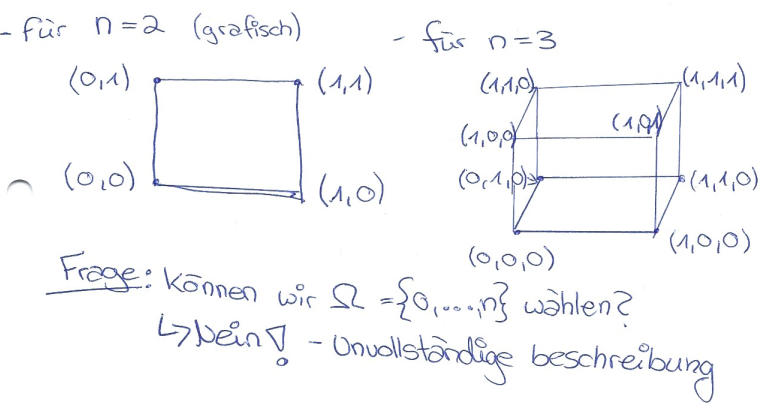
\includegraphics[width=0.8\textwidth]{img/grafikOmega.PNG}
\medskip\\
\textbf{Frage}: Können wir $\Omega = \{0,...,n\}^{n=4}$ wählen?
\section{Produktexperimente}
Betrachte n Experimente mit Grundmengen $E_1,...,E_n$\\
Führe diese Experimente unabhängig voneinander aus.\medskip\\
Grundmenge des Gesamtexperiment ist \\$\Omega = E_1\times ... \times E_n = \{(e_1,...,e_n):e_1 ß\in E_1,...,e_n\in E_n\}$\\
\#$\Omega = \#E_1 \bullet ... \bullet \#E_n$
\subsubsection{Beispiele}
\textbf{Münze und Würfel werfen}
$E_1 = \{K,Z\} \qquad E_2 = \{1,...,6\}$\\
$\Omega = E_1 \times E_2 = $\begin{tabular}{|c|c|c|c|c|c|}
	\hline 
K1	&K2  &K3  &K4  &K5  &K6  \\ 
	\hline 
Z1	& Z2 & Z3 &Z4  &Z5  &Z6  \\ 
	\hline 
\end{tabular} \\
 $\Omega$ = 12
\subsubsection{Definition: Ereignis}
Ereignis = Teilmenge von $\Omega$\\
\textbf{Beispiel}: 1 Würfel. $\Omega$ = \{1,...,6\}\\
Ereignisse: A = ''Würfel zeigt gerade Zahl'' = \{2,4,6\}\\
B = 'Primzahl gewürfelt' = \{2,3,5\}\medskip\\
\textbf{Interpretation}: Zufallsexperiment wird ausgeführt $\Rightarrow$ \\
Wir erfahren den Ausgang w $\in \Omega$\\
Sei A $\subset \Omega$. Liegt w $\in$ A, so sagen wir ''A ist eingetreten''. \\
w $\notin$ A $\Rightarrow$ ''A nicht eingetreten''\medskip\\
\textbf{Beispiel}: 2 Würfel. $\Omega = {1,...,6}^2$\\
A = ''Augensumme  = 10'' = \{(6,4),(5,5),(4,6)\}\medskip\\
Unmögliches Ereignis: $\emptyset$\\
Sicheres Ereignis (tritt immer ein) = $\Omega$\newpage
\section{Boole'sche Algebra}
Seien A $\subset \Omega$; B $\subset \Omega$\\
A $\cup$ B = \{w $\in$ $\Omega$ : w $\in$ A oder w $\in$ B\}\\
= ''mindestens ein Ereignis tritt ein.''\\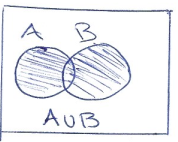
\includegraphics[width=0.2\textwidth]{img/ver.PNG}\medskip\\
A $\cap$ B = \{w $\in$ $\Omega$ : w $\in$ A und w $\in$ B\}\\
= ''beide Ereignisse treten ein.''.\\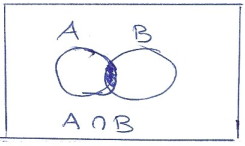
\includegraphics[width=0.2\textwidth]{img/schnitt.PNG}\medskip\\
$A^C =\{ w \in \Omega : w \notin A\}$\\
= ''A tritt nicht ein''\\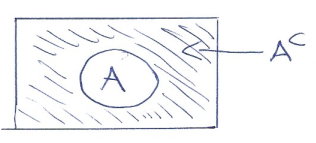
\includegraphics[width=0.3\textwidth]{img/komplement.PNG}\medskip\\
A$\backslash$B = $\{w \in \Omega : w \in A $ und $w \notin B\}$\\
= ''A tritt ein \textbf{und} B tritt nicht ein'' = $A\cap B^C$\medskip\\
B$\backslash$A = $B\cap A \subset$\\
A$\Delta$B = (A$\backslash$B)$\cup$(B$\backslash$A)\\
= ''\textbf{genau} ein Ereignis tritt ein''\\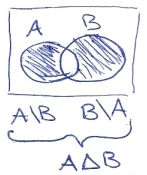
\includegraphics[width=0.2\textwidth]{img/genau1.PNG}\medskip\\
\textbf{Beispiel}: 2 Würfel $\Omega = \{1,...,6\}^2$\\
A = ''1. Würfel zeigt 6 '' = \{(6,1),(6,2),(6,3),(6,4),(6,5),(6,6)\}\\
B = ''2. Würfel zeigt 6'' = Das gleiche, nur vertauscht\medskip\\
A $\cap$ B = \{(6,6)\}\\
A $\cup$ B = \{(6,1),...,(6,6),(1,6),...,(5,6)\}
A $\Delta$ B = \{(6,1),...,(6,5),...,(1,6),...(5,6)\}\newpage
\textbf{Definition: Disjunkt}\\
Ergebnis A und B sind disjunkt, wenn A $\cap$ B = $\emptyset$\\D.h. A und B können nicht gleichzeitig eintreten.\\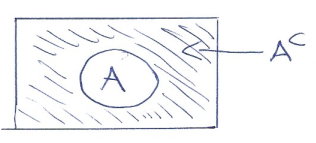
\includegraphics[width=0.3\textwidth]{img/komplement.PNG}\medskip\\
\textbf{Beispiel}: A und $A^C$,\\ A$\backslash$B,\\ A$\Delta$B,\\ und A$\cap$B sind disjunkt.\medskip\\
\textbf{Definition}: A $\subset$ B, wenn $\forall w \in A \Rightarrow w \in B$\\Wenn A eintritt, dann tritt auch B ein.\\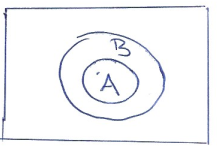
\includegraphics[width=0.3\textwidth]{img/subset.PNG}\medskip\\
\section{De Morgan-Regeln}
$\left( A \cup B\right)^C$ = ''Kein Ereignis tritt ein'' = ''A tritt nicht ein \textbf{und} B tritt nicht ein'' = $A^C \cap B^C$\\
\textbf{Regel}:$(A\cup B)^C = A^C \cap B^C$\medskip\\
$(A \cap B)^C =$''\textbf{mindestens} ein Ereignis tritt nicht ein.'' = ''A tritt nicht ein \textbf{oder} B tritt nicht ein.'' = $A^C\cup B^C$\medskip\\
\textbf{Regel}: ($A\cup B)^C$\\
\textbf{Allgemein}: \\$(A_1\cup,A_2,\cup,...)^C = A_1^C\cap A_2^C\cap...$\\
$(A_1\cap,A_2,\cap,...)^C = A_1^C\cup A_2^C\cup...$
\section{Wahrscheinlichkeiten}
\textbf{Buffon}:\\
4040 Würfe einer Münze. 2048 Kopf.\medskip\\
\textbf{Pearson}: 24000 Würfe, 12012 Kopf\medskip\\
\textbf{Rechner}:100000 Würfe, 50106 Kopf. Häufigkeit: 0,50106\\
\subsection{Empirisches Gesetz der großen Zahlen}
Betrachte Zufallsexperiment und Ereignis A $\subset \Omega$\\
Wiederhole das Experiment n Mal.\\
Zähle, wie oft A eingetreten ist: $kn(A)$ $$\frac{k_n(A)}{n} (\text{Häufigkeit}) \underset{n\rightarrow \infty}{\rightarrow} \mathds {P}[A] \text{(Wkeit von A0)}$$ 
\textbf{Definition}: Diskreter Wahrscheinlichkeitsraum ist ein Paar ($\Omega$,p), wobei $\Omega$ eine Menge ist und
$$:\Omega \rightarrow [0,1] \text{ mit } \sum_w\in \Omega p(w) = 1$$
Wahrscheinlichkeit eines Ausgangs w $\in$ Sigma ist p(w)\\
Wahrscheinlichkeit eines Ereignis A $\subset \Omega : \mathds {P}[A]=\Sigma_{w\in A}\:p(w)$\medskip\\
\textbf{Definition} Ein Laplace-Experiment liegt vor, wenn 
$$\#\Sigma = n < \infty \text{ und } p(w) = \frac{1}{n}\forall w \in \Omega[\text{Ausgänge sind gleichwahrscheinlich}]$$
Dann gilt : $$\mathds {P}[A]=\frac{\#A}{n}= \frac{\#A}{\#\Omega}$$
\textbf{Beispiel}: 2 \textbf{faire} Würfel $\Omega = \{1,...,6\}^2 \qquad \#\Omega = 36$\\
A = ''Augensumme  = 10'' = \{(6,4),(5,5),(4,6)\}
$$\mathds {P}[A] = \frac{3}{36}=\frac{1}{12}$$
B = ''Augensumme = 11'' = \{(6,5),(5,6)\} $\rightarrow \mathds {P}=\frac{1}{18}$\medskip\\
\textbf{Beispiel}: Nicht-Laplace-Experiment
\includegraphics[width=0.1\textwidth]{img/torte.PNG}\\
$\Omega = \{1,2,3\} \qquad p(1) = \frac{1}{4} \quad p(2)=\frac{1}{4} \quad p(3) = \frac{1}{2}$\\oder
$\Omega = \{1,2,3A,3B\} \Rightarrow \text{Laplace-Experiment, da} \\ p(w) = \frac{1}{4} \forall w. \mathds {P}[3] = \frac{1}{4}+\frac{1}{4} = \frac{1}{2}$\medskip\\


\chapter{Kombinatorik}
\textbf{Beispiel}: Geburtstagsproblem \hspace{1.5cm} K = 200 Personen\\
A = ''mindestens 2 Personen haben am gleichen Tag Geburtstag''\\
$\mathds{P}[A] = ?$\\\\
\textbf{Modell}: n = 365 Tage im Jahr\\\\
\textbf{Ausgänge}: Liste der Länge K besteht aus Zahlen zwischen 1 und n\medskip\\
$\Omega = \{1,...,n\}^K=\{(a_1,...,a_k):a_i \in \{1,...,365\}\forall i = 1,...,k\}$\smallskip\\
$a_i = $ Geburtstag der i-ten Person.\\
\#$\Omega =\underbrace{n*n*...*n}_K = n^K = 365^{200}$\\
$\mathds{P}[A] = \frac{\#A}{\#\Omega}$\smallskip\\
Gegenereignis $A^C$ = ''alle Geburtstage sind (paarweise) verschieden''\\\\
$\#A^C = \underbrace{n}_{\text{Mögl. für Person 1}}*\underbrace{(n-1)}_{\text{Mögl. für Person 2}}*\underbrace{(n-2)}_\text{Mögl. für 3. Person} * ... * \underbrace{(n-K+1)}_\text{Mögl. für Person k} = (n)_K$ mit K$ \leq  $n\medskip\\
$\mathds{P}[A] = \frac{\#A}{\#\Omega} = \frac{\#\Omega-\#A^C}{\#\Omega}=1-\frac{\#A^C}{\#\Omega}=1-\frac{n(n-1)...(n-K+1)}{n^K}$\medskip\\
\textbf{Beispiel}:\\ K = 23 Personen: $\mathds{P}[A]=$0.507\\K = 200: $\mathds{P}[A]=0.999999...8 \approx 1$\newpage
\section{Urnenmodelle}
Urne mit Bällen 1,...,n. Es wird k mal jeweils ein Ball zufällig gezogen. [*GRAFIK URNE]\\
\textbf{Möglichkeiten}:
\begin{enumerate}
	\item[a)] Mit/ohne Zurücklegen
	\item[b)] Nummern der Bälle mit/ohne Berücksichtigung der Reihenfolge
\end{enumerate}
Insgesamt 4 Modelle:
\begin{enumerate}
	\item \textbf{Mit Zurücklegen und mit Berücksichtigung der Reihenfolge}\\
	Ausgänge dieses Experiments sind Listen der Länge K bestehend aus Zahlen zwischen 1 und n.\\
	$\Omega=\{(a_1,...,a_k):a_i \in \{1,...,n\} \forall i = 1,..,K\}$\\
	$a_i$ = die Nummer des i-ten Ball\smallskip\\
	\textbf{Beachte}
	\begin{itemize}
		\item 	Es ist möglich, dass $a_i = a_j$ (mit Zurücklegen)
		\item 	$(5,3,7,...) \neq (3,5,7,...)$
	\end{itemize}
	\textbf{Beispiel}:
	\begin{itemize}
		\item Geburtstage von Personen. Bälle = Tage. \\Jede Person zieht einen Ball zufällig.
		\item k-maliges Würfeln. 6 Bälle = 6 Seiten des Würfels\\
	\end{itemize}
	$\#\Omega = \underbrace{n * n * ... * n}_K = n^K$
	\item \textbf{Ohne Zurücklegen und mit Berücksichtigung der Reihenfolge}\\
	$\Omega=\{(a_1,...a_k):a_i \in \{1,...,n\},\underbrace{a_i \neq a_j\forall i\neq j}_\text{Paarweise verschiedene Elemente} \}$\smallskip\\
	\#$\Omega = n* (n-1)*(n-2)*...*(n-K+1)$\smallskip\\
	\textbf{Beachte}
	\begin{itemize}
		\item (1,3,\textbf{2},4,5,\textbf{2},...) $\notin \Omega$
		\item (5,3,7,...) $\neq$ (3,5,7,...)
	\end{itemize}
	\textbf{Bemerkungen}: 
	\begin{itemize}
		\item Falls k $>$ n: \#$\Omega = 0$
		\item Für k = n:\\
		\#$\Omega = n*(n-1)*...*1 = 1*2*3*...*n = n!$\\Ausgänge sind Permutationen:\\n= 3:(1,2,3),(1,3,2),(2,1,3),(2,3,1)
	\end{itemize}
	\item \textbf{Ohne Zurücklegen und ohne Berücksichtigung der Reihenfolge}\\
	Ausgänge: Listen der Länge K aus verschiedenen Elementen.\\
	Allerdings wird die Reihenfolge nicht berücksichtigt, d.h. \{2,5,3\} = \{5,3,2\}\smallskip\\
	Ausgänge sind K-elementige Teilmengen von \{1,...,n\}.\medskip\\
	$\Omega = \{A:A\subset\{1,...,n\},|A| = k\}$ oder \\
	$\Omega = \{(a_1,...,a_k):a_i \in \{1,...,n\},\underbrace{a_1<a_2<...<a_k}_{\substack{\text{Reihenfolge wird}\\\text{ durch sortieren gelöscht}}} \}$\medskip\\
	\#$\Omega = \frac{n*(n-1)*...*(n*K+1)}{K!}$ \hspace{0.5cm}K Objekte aus n Objekten auswählen\smallskip\\
	$ = \binom{n}{k}$\medskip\\
	\textbf{Beispiel}: Lotto, 49 Kugeln. 6 Kugeln werden ohne Zurücklegen gezogen.\\ 
	Wir tippen auf eine Kombination aus 6 Nummern\smallskip\\
	A = ''Man hat alle 6 geraten'' $\mathds{P}[A] = \frac{1}{\binom{49}{6}}$\medskip\\
	\textbf{1. Lösung}:\\
	$\Omega = $ Menge aller 6-elementigen Teilmengen von \{1,...,49\}. \\
	Die Kugeln werden mit einem Griff gezogen.\medskip\\
	\#$\Omega = \binom{49}{6} \qquad \#A = 1$ [die Kombination, auf die wir tippen]\medskip\\
	$\mathds{P}[A] = \frac{1}{\binom{49}{6}} \approx 7,15*10^{-8}$\medskip\\
	\textbf{2. Lösung}:\\
	Kugeln werden einzeln gezogen, Nummern werden notiert:\\
	$\Omega = \{(a_1,...,a_6):a_i \in \{1,...,49\},a_i \neq a_i \forall i \neq j\}$\smallskip\\
	\#$\Omega = 49*48*47*...*(49-6+1) \qquad \#A = 6! $\medskip\\
	Wir tippen auf \{1,...,6\}. wir gewinnen bei allen Permutationen von 1,...,6.\\
	$\mathds{P}[A] = \frac{\#A}{\#\Omega}=\frac{6!}{49*48*...*44} = \frac{1}{\binom{49}{6}}$\medskip\\
	\textbf{Beispiel}:\\ Wie hoch ist die Chance, dass 2 mal in Folge die gleichen Zahlen gezogen werden?\\
	Bis zum Zeitpunkt gab es K = 3016 Ziehungen.\\
	Insgesamt gibt es $\binom{49}{6}$ Gewinnreihen.\medskip\\
	A = ''Bei mindestens 2 Ziehungen wurde die gleiche Reihe gezogen''\\$\approx$ Geburtstagsproblem\medskip\\
	$A^C = $ ''Alle Ziehungen ergeben verschiedene Reihen''\medskip\\
	$\mathds{P}[A] = 1 - \frac{n(n-1)...(n-K+1)}{n^K}$ = 0,278\medskip\\
	$\Rightarrow$ \textbf{Ferni-Dirar-Statistik}
	\newpage
	\item \textbf{Mit zurücklegen und ohne Reihenfolge}\\
	K Vögel setzen sich auf n Bäume
	\begin{itemize}
		\item 	Mehrfachbesetzungen möglich
		\item 	Vögel identisch
	\end{itemize}
	\textbf{Wieviele Besetzungen sind möglich?}\medskip\\
	\textbf{Lösung}:\\
	Insgesamt $\underbrace{K}_\text{Vögel}+\underbrace{n-1}_\text{''Trennwände''}$ Symbole, davon K Kreuze\medskip\\
	\#$\Omega = \binom{K+n-1}{K} = \binom{K+n-1}{n-1} $\medskip\\
	$\binom{a}{b} = \binom{a}{a-b}$\smallskip\\
	$\Rightarrow$ Bose-Einstein-Statistik (für diese Vorlesung unwichtig)
\end{enumerate}


\section{Binomialkoeffizient}
\textbf{Def.:} Binomialkoeffizient $\binom{n}{k}$ ist die Anzahl der k-elementigen Teilmengen von \{1,..,n\}\medskip\\
 $$\text{\textbf{Formel: }}\binom{n}{k}= \frac{n*(n-1)*...*(n-k+1)}{k!}$$
 $$=\frac{n!}{(n-k)!*k!}$$ k $\in$ \{0,...,n\}\smallskip\\
\textbf{ Wieso teilen wir durch (k!)?}\\
 Weil jede k-elem. Teilmenge k!-mal gezählt wurde. Z.B. \{3,5,9\} als (3,5,9), (3,9,5),...\\
 \textbf{Bsp.:} 20 Schüler.\\Es soll eine Fußballmanschafft gebildet werden.\\
 Anz. der Mögl. ohne Berücksichtigung der Positionen: $\binom{20}{10}$\medskip\\
 \textbf{Bsp.:} 52 Karten, davon 4 Asse. Wir ziehen 4 Karten ohne zurücklegen. Wkeit, dass alle 4 Asse sind\\
 $\Omega$ = 4-elem. Teilmengen von \{1,...,52\}\\
 \#A=1 \hspace{1cm} $\mathds{P}[A]=\dfrac{\#A}{\Omega}=\dfrac{1}{\binom{52}{4}}=3,7*10^{-6}$\medskip\\
 \textbf{Bsp.:} 52 Karten, 4 werden gezogen.\\
 A = ''Alle sind Pik''
 $\mathds{P}[A]= ? \qquad \#A=\binom{13}{4} $\\
 \#$\Omega = \binom{52}{4} \qquad \mathds{P}[A] = \dfrac{\binom{13}{4}}{\binom{52}{4}} \approx 2,64*10-{-3} $\medskip\\
 \textbf{Satz 3.1}:\\ Wenn 0 $\leq$ k $\leq$n-1\\
 $=\binom{n}{k}=\binom{n-1}{k}+\binom{n-1}{k-1}$\smallskip\\
 \textbf{Bew.:} Wir wollen aus n Elem. k auswählen.\\
 2 Fälle:
 \begin{enumerate}
 	\item Wir haben das Element ''n'' ausgewählt. \\ Es verbleiben n-1 Elem, von denen k-1 ausgewählt werden sollen.$\binom{n-1}{k-1}$ Mögl.
 	\item Wir haben das Elem. ''n'' nicht ausgewählt.\\
 	Es verbleiben n-1Elem., von denen k ausgewählt werden sollen $\binom{n-1}{k}$ Mögl.
 \end{enumerate}
\section{Bin. Lehrsatz}
$(x+y)^0=1$\\
$(x+y)^1 = x+y$\\
$(x+y)^2 = x^2+2xy+y^2$\\
$(x+y)^3= x^3+3x^2y+3xy^2+y^3$\medskip\\
$(x+y)^n=x^n+\binom{n}{1}x^{n-1}y+\binom{n}{2}x^{n-2}y^2+...+y^n$[GRAFIK PASCALSCHE DREICECK]\medskip\\ 
\textbf{Satz 3.2.}:\\
$(x+y)^n =\sum^n_{k=0} \binom{n}{k}x^ky^{n-k}$\medskip\\
\textbf{Bew.}: \\
Beim Ausmultiplizieren zählen wir, wie oft der Term $x^ky^{n-k}$ entsteht.\\
Aus k Faktoren muss x als Beitrag ausgewählt werden, aus dem Rest y.
$(x+y)^n=(x+y)(x+y)*...*(x+y)$\\
$\binom{n}{k}$ Mögl. \qed\medskip\\
\textbf{Bem.:} $\binom{n}{k}=\binom{n}{k-1}$, d.h. jede (Spalte vom Pascal'schen Dreieck) liest sich von rechts genauso wie von links.\\
k Elem. auswählen $\Leftrightarrow$ n-k nicht auswählen.\\
 \textbf{Beobachtung}: Zeilen summieren im Pascal'schen Dreieck: Zeilen summieren im Pascal'schen Dreieck: Summe ist $2^n$\medskip\\
 \textbf{Satz 3.3}: $\sum^n_{k=0} \binom{n}{k} = 2^n$\\
 \textbf{Bew.:}\\
 $\sum^n_{k=0}\binom{n}{k}1^k1^{n-k} = (1+1)^n=2^n\qed$\\
 \textbf{Übung: Ähnlich}:\\
 $\binom{n}{0}+\binom{n}{2}+\binom{n}{4}+...=\binom{n}{1}+\binom{n}{3}+\binom{n}{5}+...$\medskip\\
\subsection{ Pasal'sche Dreieck und Trigonometrie}
\begin{tabbing}
	Bekannt: \= $\sin(2) = 2\sin x \cos x$\\
	\> $\cos(2x)=\cos^2x-\sin^2x$
\end{tabbing}
Es gibt auch Formeln für $\sin(3x) , \cos(3)$,...\medskip\\
(GRAFIK FORMELN $\cos(...)$)\\
\textbf{Allgemein}:\\
$\sin(nx) = \binom{n}{1}\cos^{n-1}(x) \sin x - \binom{n}{3}\cos^{n-1}x \sin^3x + \binom{n}{5} \cos^{n-5}x \sin^5x-...$\medskip\\
$\cos(nx) = \cos^nx - \binom{n}{2}\cos^{n-2}x\sin^2x+\binom{n}{4}\cos^{n-4}x\sin^4x-...$\medskip\\
Bew.: Induktion (Übung YAAAY)
\section{Hypergeometrische Verteilung}
\begin{tabbing}
	Teich mit n Fischen:\hspace{1cm}\= $n_1$ Fische rot\\
	$n_1 + n_2 = n$ \>$n_2$ Fische gelb
\end{tabbing}
Fischer fängt k Fische (Ohne Zurücklegen).\\
k$\leq$n\medskip\\
A=''$k_1$ rote und $k_2$ gelbe Fische gefangen.''\\
$k_1 + k_2 = k$\medskip\\
$\mathds{P}[A] = ?$\smallskip\\
\textbf{Lösung:} $\Omega$ = \{T $\subseteq$ \{1,...,n\}, \#T = k\}\hspace{5mm} \#=$\binom{n}{k}$\medskip\\
A: Aus $n_1$ roten Fischen $k_1$ ausw. $\binom{n_1}{k_1}$\\
Aus $n_2$ gelben Fischen $k_2$ ausw. $\binom{n_2}{k_2}$\\
Diese sind beliebig kombinierbar.\\
Insgesamt: \#A = $\binom{n_1}{k_1}*\binom{n_2}{k_2}$\\
$\mathds{P}[A] = \dfrac{\binom{n_1}{k_1}*\binom{n_2}{k_2}}{\binom{n}{k}}$\medskip\\
\textbf{Bsp.:} Lotto: 6 aus 49\\
$\mathds{P}$[''$\underbrace{\text{Man hat \textbf{genau} 3 richtig}}_{=A}$'']\\
\textbf{Lösung:}\\
$\Omega = \{T \subseteq \{1,...,49\},|T| = 6\} \qquad \#\Omega = \binom{49}{6}$\\
 Ohne Einschränkung tippen wir auf \{1,...,6\} damit A eintritt:
\begin{itemize}
\item Es müssen 3 Kugeln aus \{1,...,6\} gezogen werden: $\binom{6}{3}$ Mögl.
\item Es müssen 3 Kugeln aus \{7,...,49\} gezogen werden $\binom{43}{3}$ Mögl.\\
\#A = $\binom{6}{3}*\binom{43}{3}$\smallskip\\
$\mathds{P}[A] = \dfrac{\binom{6}{3}*\binom{43}{3}}{\binom{49}{6}}\approx 0,0176$
\end{itemize}

\section{Touren}
\begin{enumerate}
	\item 5 Städte aus 12 Städten für eine Rundreise auswählen.\\
	\# Touren = ?
	\begin{tabbing}
		\textbf{Lösung:} \=12 Möglichkeiten für Startpunkt\\
		\> 11 Möglichkeiten für die nächste Stadt usw.
	\end{tabbing}
	\textbf{Insgesamt}: $12*11*10*9*8$ Möglichkeiten
	\item 12 Personen, Ausschuss aus 5 Personen, darunter 1 Vorsitzender\\
	\# Möglichkeiten = ?\medskip\\
	\textbf{Lösung 1:} $\underbrace{\binom{12}{5}}_\text{Vositzenden auswählen} * \:5$\medskip\\
	\textbf{Lösung 2:} $\underbrace{12}_\text{Vorsitzender} *\: \binom{11}{4}$
\end{enumerate}
\newpage
\section{Allgemeine hypergeometrische Verteilung}
Teich mit n Fischen und r möglichen Farben:\medskip\\
$n_1$ Fische haben Farbe 1, \hspace{1cm} $n_1 + n_2 +...+n_3 = n$\\
...\\
$n_r$ Fische haben Farbe r\medskip\\
Fischer fängt K Fische\\
A = ''genau $k_1$ Fische mit Farbe 1 gefangen, ... , genau $k_r$ Fische mit Farbe r gefangen'' mit $k_1 + ... + k_r = k$\medskip\\
$\mathds{P}[A] = ?$\medskip\\
\textbf{Lösung:} $\Omega = \{ T \subset \{1,...,n\}:\#T=k\} \qquad \#\Omega = \binom{n}{k}$\medskip\\
$\#A = \binom{n_1}{k_1} * \binom{n_2}{k_2}*...*\binom{n_r}{k_r}$\medskip\\
$k_1$ Fische mit Farbe 1 auswählen: $\binom{n_1}{k_1}$\\
$k_r$ Fische mit Farbe r auswählen: $\binom{n_r}{k_r}$\medskip\\
$\mathds{P}[A] = \underbrace{\dfrac{\binom{n_1}{k_1}*...*\binom{n_r}{k_r}}{\binom{n}{k0}}}_\text{Allgemeine hypergeometrische Verteilung}$\medskip\\
\textbf{Beispiel}: 52 Karten\\
Zufällig auf 2 Spieler verteilt. Jeder Spieler bekommt 26 Karten.\medskip\\
A = ''Spieler 1 bekommt genau 3 Asse, 2 Könige und 1 Dame'\smallskip'\\
$\mathds{P}[A] = ?$\medskip\\
\textbf{Lösung:} $\#\Omega = \binom{52}{26} * \underbrace{\binom{26}{26}}_{=1}$\medskip\\
$\#A=\underbrace{\binom{4}{3}}_\text{3 A aus 4}*\underbrace{\binom{4}{2}}_\text{2 K aus 4}*\underbrace{\binom{4}{1}}_\text{1 D aus 4}*\underbrace{\binom{40}{20}}_{\substack{\text{aus 40 verbl.}\\\text{ Karten 20 auswählen}}}$\medskip\\
\textbf{Beispiel:} Zug mit 10 Waggons, jeweils 50 Plätze.\\
30 Personen suchen sich zufällig Plätze aus\smallskip\\
A = ''in jedem Waggon genau 3 Personen''\medskip\\
\textbf{Lösung:} $\#\Omega = \binom{500}{30}$ [30 Plätze ausgewählt, die besetzt werden sollen]\medskip\\
$\#A = \underbrace{\binom{50}{3}*\binom{50}{3}*...*\binom{50}{3}}_10 = \binom{50}{3}^{10}$\smallskip\\
$\mathds{P}[A] = \dfrac{\binom{50}{3}^{10}}{\binom{500}{30}}$
\section{Multinomialkoeffizient}
\textbf{Beispiel}: k verschiedene Gegenstände sollen auf r Fächer verteilt werden, s.d.:\\
Im 1. Fach $k_1$ Gegenstände landen, \hspace{1cm} $k_1 +k_2+ ... + k_r = k$\\
Im 2. Fach $k_2$ Gegenstände landen,\\...\\
Im r. Fach $k_r$ Gegenstände landen\smallskip\\\# Möglichkeiten = ?\medskip\\
\textbf{Lösung:}\\
Wähle $k_1$ Gegenstände für Fach 1: $\binom{k}{k_1}$\smallskip\\
Wähle $k_2$ Gegenstände für Fach 2: $\binom{k-k_1}{k_2}$\smallskip\\
Wähle $k_3$ Gegenstände für Fach 3: $\binom{k-k_1-k_2}{k_3}$\\
...\\
Wähle $k_r$ Gegenstände für Fach r: $\binom{k-k_1-k_2-...-k_{r-1}}{k_r} = \binom{k_r}{k_r} = 1$\medskip\\
Insgesamt: $\binom{k}{k_1}*\binom{k-k_1}{k_2}*\binom{k-k_1-k_2}{k_3}*...*\binom{k-k_1-k_2-...-k_{r-1}}{k_r} = \\\dfrac{k!}{k_1!*k_2!*...*k_r!}$\medskip\\
$k! = 1 * 2 * ... * k$\\
$1! = 1$\\
$0! = ! \qquad \binom{n}{n} = \dfrac{n!}{n!*0!}=\dfrac{1}{0!}=1$
\subsubsection{Definition: Multinomialkoeffizient}
$\binom{k}{k_1,k_2,...,k_r} := \dfrac{k!}{k_1!*k_2!*...*k_r!}$\medskip\\
Spezifalfall: r = 2:\medskip\\
$\binom{k}{k_1,k-k_1}=\dfrac{k!}{k_1!(k-k_1)!} = \binom{k}{k_1}= \binom{k}{k-k_1}$\\\\
\textbf{Multinomialformel: } $$\underbrace{(x+y+z+t)^n = (x+y+z+t)*(x+y+z+t)*...*(x+y+z+t)}_\text{n Mal}$$ 
$$=\Sigma x^{k_1}y^{k_2}z^{k_3}t^{k_4} \qquad k_1, k_2, k_3, k_4 \in \{0,1,...\}, k_1 + ... k_4 = n$$\medskip\\
\textbf{Beispiel:} Aus 33 Schülern sollen 3 Fußballmannschaften gebildet werden.\\
\#Mögl = ?\medskip\\
\textbf{Lösung}: $\binom{33}{11,11,11}= \dfrac{33!}{11!11!11!}$ [falls Mannschaften unterscheidbar]\medskip\\
Wenn Mannschaften \textbf{nicht} unterscheidbar sind: $\binom{33}{11,11,11}/3!$\bigskip\\
\textbf{Beispiel:} Wie viele 16-stellige Zahlen kann man mit einem Ziffernvorrat von \textbf{3 Einsen}, \textbf{5 Dreien} und \textbf{8 Sechsen} schreiben? \medskip\\
1,1,1,3,3,3,3,3,6,6,6,6,6,6,6,6\medskip\\
\textbf{Lösung:} 16 Stellen \qedsymbol \qedsymbol \qedsymbol ... \qedsymbol\\
3 Stellen auswählen, die mit Einsen besetzt werden. $\binom{16}{3}$\\
Es verbleiben 13 Stellen. 5 Stellen auswählen, die mit Dreien besetzt werden $\binom{13}{5}$\\
Es verbleiben 8 Stellen. Es bleibt nur eine Möglichkeit für die 8 Sechsen.\medskip\\
\textbf{Insgesamt:} $\binom{16}{3}*\binom{13}{5}*1 = \binom{16}{3,5, 8} = \dfrac{16!}{3!5!8!}$\smallskip\\
Fächer: 1,3,6\\
Gegenstände: Stellen
\subsection{Multinomialverteilung mit Zurücklegen}
\textbf{Beispiel:} Fische mit $n = \underbrace{n_1}_\text{Farbe 1}+,..,n_r$\medskip\\
Fischer fängt k Fische \textbf{mit Zurücklegen}
\begin{tabbing}
	A = ''\= genau $k_1$ Fische mit Farbe 1 gefangen,\\
	\> ...\\
	\> genau $k_r$ Fische mit Farbe r''
\end{tabbing}
$\mathds{P}[A] = ?$\medskip\\
\textbf{Lösung:} $\Omega = \{1,...,n\}^k \qquad \#\Omega = n^k$\\
Betrachte Ereignis:
\begin{itemize}
	\item Zuerst weise jeder Ziehung eine Farbe zu, s.d. $\forall i \in $ \{1,..,r\} Farbe i genau $k_i$ Ziehungen zugeordnet wird.\\Mögl.:$\binom{k}{k_1,k_2,...,k_r}$
	\item Bei gegebenen Farben ordnen wir nun jeder Ziehung einen Fisch zu.
\end{itemize}
A besteht aus $\binom{k}{k_1,...,k_r}$ ''Kopien'' von B, somit
$$\#A = \binom{k}{k_1,...,k_r}*n_1^{k_r}*...*n_r^{k_r}$$
\begin{tabbing}
	B = \= ''bei Ziehungen $1,...,k_n$ Farbe 1 gezogen,\\
	\> bei Ziehungen $k_1+1,...,k_1+k_2$: Farbe 2,\\
	\>...\\
	\> bei Ziehungen $k_1+...+k_r+1,...,k$ : Farbe r''
\end{tabbing}
$\#B=\underbrace{n_1*...*n_1}_{k_1}*\underbrace{n_2*...*n_2}_{k_2}*...*\underbrace{n_r*...*n_r}_{k_r} = n_1^{k_1}*...*n_r^{k_r}$\medskip\\
$\mathds{P}[A] = \dfrac{\#A}{\#\Omega}= \binom{k}{k_1,...,k_r}*\left(\dfrac{n_1}{n}\right)^{k_1}*\left(\dfrac{n_2}{n}\right)^{k_2}*...*\left(\dfrac{n_r}{n}\right)^{k_r}$\qed\\\\
\textbf{Beispiel:} Eine faire Münze wird n mal geworfen.\medskip\\ $\mathds{P}[\text{k Mal ''Kopf''}]= \dfrac{\binom{n}{k}}{2^n}$, dann: 
$$\#\Omega = \{Z, K\}^n\quad \#\Omega = 2^n\quad \#A=\binom{n}{k} \quad \substack{\text{[Auswahl von k Würfen,}\\\text{ in denen Kopf geworfen wurde]}}$$\\
\textbf{Zwei Aufgaben}:
\begin{enumerate}
	\item Rundreise. Kunde darf 5 aus 12 verschiedenen Städten auswählen.\\Anzahl der Touren: 12*11*10*9*8, nicht $\binom{12}{5}$ [Tour geordnet]
	\item 12 Personen. Es soll ein Ausschuss aus 5 Personen gebildet werden, davon 1 Vorsitzender. Anzahl der Mögl: $\binom{12}{5}*5$, oder $12*\binom{11}{4}$\end{enumerate}

\chapter{Axiome der WTheorie}
$\Omega$ = Menge aller Ausgänge eines Zufallsexp.\\
Ereignisse = Teilmengen von $\Omega \quad A \subset \Omega$\\
$\mathcal{P}(\Omega)$ = Menge aller Ereignisse = Potenzmenge von $\Omega \quad \#\mathcal{P}(\Omega)=2^{\#\Omega}$\\
Wahrscheinlichkeit ist eine Fkt. $\mathds{P}:\mathcal{P}(\Omega) \rightarrow [0,1] \\ A \rightarrow \mathds{P}[A] $ mit 
\begin{itemize}
	\item $\mathbf{A_1} \mathds{P}[A_1\cup A_2\cup...]=\mathds{P}[A_1]+\mathds{P}[A_2]+...$\\
	$\forall A_1, A_2,... \subset \Omega $mit $A_i \cap A_j = \emptyset$\\$\forall i \neq j$
	\item $\mathds{P}[\Omega]=1$
\end{itemize}
\section{Eigenschaften von $\mathds{P}$}
\begin{enumerate}
	\item $\mathds{P}[\emptyset]=0$
	\item $\forall A_1,...,A_n \subset \Omega $ mit $A_i \cap A_j = \emptyset \quad \forall i \neq j$\\
	$\mathds{P}[A_1\cup,...,\cup A_n] = \mathds{P}[A_1]+...+\mathds{P}[A_n]$\medskip\\
	\textbf{Spezialfall}: Für A,B $\subset \Omega$ mit A $\cap B = \emptyset$\\gilt 
	$\mathds{P}[A\cup B] = \mathds{P}[A] + \mathds{P}[B]$
	\item $\forall A \in \Omega \quad \mathds{P}[A^C]=1-\mathds{P}[A]$
	\item $\forall A, B \subset \Omega : \mathds{P}[A\backslash B] =\mathds{P}[A]-\underbrace{\mathds{P}[A\cap B]}_{\text{Nicht }\mathds{P}[B]}$
	\item A,B $\subset \Omega$ (nicht disjunkt)\\
	$\mathds{P}[A\cup B] = \mathds{P}[A] + \mathds{P}[B] - \mathds{P}[A\cap B]$
	\item Siebformel oder Einschluss-Ausschluss-Formel.\\
	\end{enumerate}

	\textbf{Für 3 Ereignisse A, B, C} $\subset \Omega \quad \mathds{P}[A\cup B \cup C]=
	\\\mathds{P}[A]+\mathds{P}[B]+\mathds{P}[C]-\mathds{P}[A\cap B] - \mathds{P}[B \cap C]-\mathds{P}[C\cap A] + \mathds{P}[A\cap B \cap C]$\medskip\\
	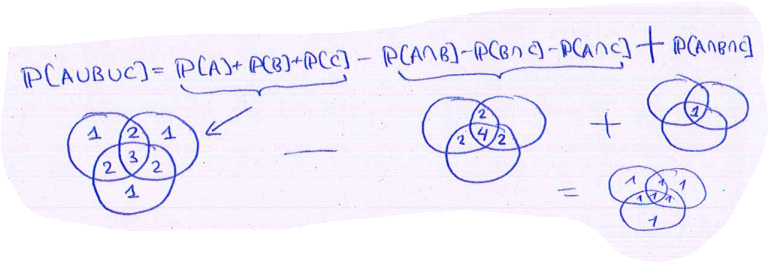
\includegraphics[width=0.8\textwidth]{img/sieb.PNG}\medskip\\
	\textbf{Für 4 Ereignisse A,B,C,D}\\
	$\mathds{P}[A]+\mathds{P}B+\mathds{P}[C]+\mathds{P}[D]$
	$-(\mathds{P}[A\cap B]+\mathds{P}[A\cap C ]+...+\mathds{P}[C\cap B]) $\smallskip
\\	$+ (\mathds{P}[A \cap B \cap C ] + \mathds{P}[B \cap C \cap D]+...)$
	$-\mathds{P}[A\cap B \cap C \cap D]$\medskip\\
	\textbf{Für n Ereignisse} $A_1,A_2,...,A_n$:\\
	$\mathds{P}[\bigcup^n_{k=1}A_k]=\Sigma^n_{i=1}\mathds{P}[A_i]-\Sigma_{1\leq i < j \leq n}\mathds{P}[A_i\cap A_j]+\Sigma_{1\leq i < j<k\leq n} \mathds{P}[A_i\cap A_j\cap A_k]- ... $\smallskip\\
	$+ (-1)^{n+1}\mathds{P}[A_1\cap ... \cap A_n]$\medskip\\
	\textbf{Bsp.:}\\
n Briefe werden zufällig in n adressierte Briefumschläge gesteckt.\\
A=''mind. 1 Brief wird in den richtigen Umschlag gesteckt''\\
$\mathds{P}[A] = ?$\medskip\\
\textbf{Lösung.:} \hspace{3cm} Briefe 1,2,3,4,5,6\\
$\Omega = \{\underbrace{(a_1,...,a_i)}_{\substack{a_i\text{ gibt an, in welchen}\\\text{ Umschlag Brief i gesteckt wird}}}: a_i \in \{1,...,n\} a_i \neq a_j \forall i \neq j \}$\medskip\\
\#$\Omega = n*(n-1)*...+1=n! \quad \#A = ?$\\
A = \{$(a_1,...,a_n)\in \Omega: \exists k \text{ mit } A_k = k$\}\medskip\\
A = $A_1\cup ...\cup A_n$ mit \\
$A_k$ = ''Brief k wird in Umschlag k gesteckt''\medskip\\
$\mathds{P}[A_k] = \dfrac{\#A_k}{\#\Omega}=\dfrac{(n-1)!}{n!} = \dfrac{1}{n}$\smallskip\\
$A_1,...,A_n $ nicht disjunkt.\\
$\mathds{P}[A_1\cap A_2] = \dfrac{\#(A_1 \cap A_2)}{n!} = \dfrac{(n-2)!}{n!}$\medskip\\
$\mathds{P}[A_1\cap A_2\cap A_3]=\dfrac{\#(A_1 \cap A_2 \cap A_3)}{n!} = \dfrac{(n-3)!}{n!}$\medskip\\
\textbf{Allgemein}: $ \mathds{P}[A_{i1}\cap A_{i2}\cap...\cap A_{il}]=\dfrac{(n-l)!}{n!}$\smallskip\\
\textbf{Siebformel}: $\mathds{P}[A] = \mathds{P}[A_1\cup ... \cup A_n]= n * \frac{1}{n}- \binom{n}{2}*\dfrac{(n-2)!}{n!}+\dfrac{(n-3)!}{n!}-...$\medskip\\
$= \Sigma_{l=1}^n \binom{1}{l}*\dfrac{(n-l)!}{n!}*(-1)^{l+1}= \Sigma_{l=1+n}^n\dfrac{(-1)^{l+1}}{l!}$ \medskip\\
$=1-\dfrac{1}{2!}+\dfrac{1}{3!}-\dfrac{1}{4!}+...+(-1)^{n+1}\dfrac{1}{n!}$\medskip\\
Für $n\rightarrow\infty  \quad \underset{n\rightarrow\infty}{\text{lim}}\mathds{P}[A]= 1-\dfrac{1}{2!}+\dfrac{1}{3!}-\dfrac{1}{4!}+... $\smallskip\\
$= 1- (\dfrac{1}{2!}-\dfrac{1}{3!}+...)= 1 - \dfrac{1}{e} \approx 0.632$

\section{Ungleichungen für Wkeiten}
$\mathds{P}[\Omega] = 1$\\
$\mathds{P}[A_1\cup A_2 \cup ...] = \mathds{P}[A_1] + \mathds{P}[A_2]+ ...$\\
falls $A_i \cap A_j = \emptyset \: \forall i+j$\medskip\\
\textbf{7.}:\\
$\forall  A \subset B \subset \Omega \Rightarrow \mathds{P}[A] \leq \mathds{P}[B]$\\
\textbf{Bew.}: $B=A\cup(B\backslash A)$ (disjunkt)\\
$\mathds{P}[B]=\mathds{P}[A]+\underbrace{\mathds{P}[B\backslash A]}_{\geq 0} \geq \mathds{P}[A] \qed$\medskip\\
\textbf{8.}:\\
$\forall A, B \subset \Omega : \mathds{P}[A\cup B] \leq \mathds{P}[A] + \mathds{P}[B]$\medskip\\
\textbf{Allgemeiner}: $\forall A_1,...,A_n \subset \Omega : \mathds{P}[A_1\cup ...\cup A_n] \leq \mathds{P} [A_1]+...+\mathds{P}[A_n]$\medskip\\
\textbf{9. } Noch allgemeiner:\\
$\forall A_1,A_2,... \subset \Omega : \mathds{P}[\bigcup_{k=1}^\infty A_k] \leq \Sigma_{k=1}^\infty \mathds{P}[A_k]$\\
\textbf{Bew.}:\\
$B_1 = A_1$\\
$B_2 = A_2\backslash A_1$\\
$B_3 = A_3\backslash(A_1 \cup A_2)$\\
...\smallskip\\
Dann gilt:\\
$\underbrace{\bigcup_{k=1}^\infty A_k}_\text{Nicht disj.} = \underbrace{\bigcup_{k=1}^\infty B_k}_\text{disj.!!!}$\medskip\\
$\mathds{P}[\bigcup_{k=1}^\infty A_k] = \mathds{P}[\bigcup_{k=1}^\infty B_k] \overset{\text{Axiom}}{=}\Sigma_{k=1}^\infty \mathds{P}[B_k] \underset{B_k \subset A_k}{\leq} \Sigma_{k=1}^\infty \mathds{P}[A_k] \qed$
\chapter{Bedingte Wahrscheinlichkeiten und Unabhängigkeiten}
\textbf{Bsp.}: 2 faire Würfel \hspace{1cm} $\Omega = \{1,...,6\}^2 \quad \#\Omega=36$\\
A= 'Erster Würfel zeit eine 6''\hspace{1cm} B=''Augensumme = 10''\smallskip\\
Jemand teilt uns mit: B ist eingetreten.\smallskip\\
$A=\{(6,1),(6,2),...,(6,6)\} \quad \#A =6 \quad \mathds{P}[A] = \frac{6}{36}= \frac{1}{6}$
$B=\{\underbrace{(6,4)}_\text{A tritt ein},(5,5),(4,6)\}$\medskip\\
$\mathds{P}[A|B]= \frac{1}{3}$\medskip\\
\textbf{Definition}:\\
Seien $A,B \subset \Omega$. Bedinge Wkeit von A gegeben B ist: $$\mathds{P}[A|B] = \dfrac{\mathds{P}[A \cap B]}{\mathds{P}[B]}$$
Annahme: $\mathds{P}[B] \neq 0$\medskip\\
\textbf{Bsp.}:\\ Fairer Würfel wird 10x geworfen.\\
Uns wird mitgeteilt, dass mindestens eine 6 gewürfelt wurde.\smallskip\\
Bedingte Wkeit, dass der erste Wurf eine 6 war = ?\medskip\\
\textbf{Lösung}:\\
$\Omega = \{(a_1,...,a_{10}):a_i \in \{1,..,6\}\} \quad \#\Omega = \overbrace{6*6*...*6}^{10} = 6^{10}$\\
B = ''mind. eine 6 gewürfelt'' \hspace{1cm} $B^C =$ ''keine 6 gewürfelt'' =\\
$\{(a_1,...,a_10):a_i \in \{1,2,...,5\}\} \quad \#B^C = 5^{10}$\smallskip\\
$\#B = 6^{10}-5^{10}$\\
$\mathds{P}[B] = \dfrac{6^{10}-5^{10}}{6^{10}}$\smallskip\\
A = '' der erste Wurf ist eine 6''\\
$A = \{(6,a_2,...,a_10):a_i \in \{1,...,6\}\}$\\
$\#A = \underbrace{1*6*6*...*g}_9 = 6^9	$\smallskip\\
$\mathds{P}[A] = \dfrac{6^9}{6^{10}}= \dfrac{1}{6}$\medskip\\
$A\cap B = A$\\
$\mathds{P}[A\cap B] = \mathds{P}[A]=\frac{1}{6}$\smallskip\\
$\mathds{P}[A  \vert B ] = \dfrac{\mathds{P}[A \cap B]}{\mathds{P}[B]} = \dfrac{6^9}{6^{10}-5^{10}} = 0,19$\medskip\\
$\mathds{P}[A\vert B] = 0,19$\\
$\mathds{P}[A] = 0,16$\medskip\\
\textbf{Alternativ}: $\mathds{P}[A\vert B] = \dfrac{\#(A\cap B)}{\#B}$\medskip\\
\section{Eigenschaften der bedingten Wkeiten}
\begin{enumerate}
	\item $\mathds{P}[A \vert B] = \dfrac{\mathds{P}[A \cap B]}{\mathds{P}[B]} \leq 1 $ (und $\geq 0$)
	\item $\mathds{P}[\Omega\vert B] = \dfrac{\mathds{P}[\Omega \cap B]}{\mathds{P}[B]}= \dfrac{\mathds{P}[B]}{\mathds{P}[B]} = 1$
	\\ $\mathds{P}[\emptyset \vert B] = 0$
	\item Falls $A_1,A_2,...$ disj. sind, gilt:
	$$\mathds{P}\left[\left(\bigcup_{k=1}^\infty A_k\right)\vert B\right] = \Sigma_{k=1}^\infty \overset{\text{Def.}}{=} \dfrac{\mathds{P}\left[\left(\bigcup_{k=1}^\infty A_k\right)\cap B\right]}{\mathds{P}[B]}$$
	$$= \dfrac{\mathds{P}\left[\bigcup_{k=1}^\infty(A_k \cap B)\right]}{\mathds{P}[B]}$$
	$$\overset{A_\cap B ,A_2 \cap B,... \text{disj}}{=} \dfrac{\Sigma_{k=1}^\infty \mathds{P}[A_k \cap B]}{\mathds{P}[B]} = \Sigma_{k=1}^\infty \dfrac{\mathds{P}[A_k \cap B]}{\mathds{P}[B]} = \Sigma_{k=1}^\infty \mathds{P}[A_k \vert B] \qed$$
	\item $\mathds{P}[A^C\vert B] = 1 - \mathds{P}[A\vert B]$
	\item Multiplikationsregel:\\$\mathds{P}[A_1\cap A_2] = \mathds{P}[A_1]*\mathds{P}[A_2\vert A_1]$\smallskip\\
	$\mathds{P}[A_1\cap A_2\cap A_3] = \mathds{P}[A_1] * \mathds{P}[A_2 \vert A_1]* \mathds{P}[A_3 \vert (A_1 \cap A_2)]$\smallskip\\
	\textbf{Sterbewahrscheinlichkeiten $q_0,q_1,...$}\\
	$q_n = $ Wahrscheinlichkeit, als eine n-jährige Person, dass Alter n+1 nicht zu erreichen.\smallskip\\
	$q_0 = 0,0046$ \hspace{2cm} Wkeit, dass eine Person $\geq$ 50 alt wird\\
	$q_1 = 0,0004$\\
	$q_2 = 0,0002$\smallskip\\
	\textbf{Lösung}: Def.: $A_n$=''Person hat das Alter von n Jahren erreicht''\\$\mathds{P}[A_{50}] = ?$\medskip\\
	Gegeben sind $q_n = \mathds{P}\left[A_{n+1}^C \vert A_n\right]\quad 1-q_n = \mathds{P}[A_{n+1}\vert A_n]$\\
	$\mathds{P}[A_{50}] = \mathds{P}[A_1]*\mathds{P}[A_2 \vert A_1]*\mathds{P}[A_3\vert (A_1 \cap A_2)]*\mathds{P}[A_4 \vert \underbrace{(A_1 \cap A_2 \cap A_3)}_{A_3}] * ... * \mathds{P}[A_{50}\vert \underbrace{(A_1\cap...\cap A_{49})}_{A_{49}}] $\\ $=(1-q_0)*(1-q_1)*...*(1-q_{49})$\medskip\\
	$\mathds{P}[\text{Person lebt genau 50 Jahre}] =(1-q_0)*(1-q_1)*...*(1-q_{49}) * q_{50}$\qed
\end{enumerate}


\section{Unabhängige Ereignisse}
%\textbf{Definition}: ER. A und B heißen unabhängig, wenn $$\mathds{P}[A\cap B] = \mathds{P}[A] - \mathds{P}[B]$$
%A, B unabhängig $\Rightarrow$\\
%$\mathds{P}[A\vert B] = \mathds{P}[A]$\medskip\\
%\textbf{Bsp.}:\\
%1 fairer Würfel\\
%A= ''gerade Zahl gewürfelt'' = \{2,4,6\}\\
%B = ''Augenzahl $\geq$ 5'' = \{5,6\}\medskip\\
%$\mathds{P}[A] = \frac{1}{2}..:$
Zwei Formeln:
\begin{enumerate}
	\item $\mathds{P}[A\cup B] = \mathds{P}[A]+\mathds{P}[B] \quad$, falls A $\cap$ B = $\emptyset$
	\item $\mathds{P}[A\cap B] = \mathds{P}[A]*\mathds{P}[B] \quad$, falls A und B unabhängig
\end{enumerate}
\textbf{Bemerkung}: Disjunkt und unabhängig sind verschiedene Begriffe.\smallskip\\
Seien A, B disjunkt (d.h. A $\cap$ B = $\emptyset$)\medskip\\ $\Rightarrow \mathds{[\underbrace{A \cap B}_\emptyset]}= 0 \neq \mathds{P}[A]*\mathds{P}[B]$\smallskip\\$\Rightarrow$ A und B abh. (Falls $\mathds{P}[A], \mathds{P}[B] \neq 0$\medskip\\
\textbf{Definition}:\\
Ereignisse A,B,C heißen
\begin{itemize}
	\item paarweise unabhängig, wenn $\mathds{P}[A\cap B] = \mathds{P}[A]*\mathds{P}[B],\: \mathds{P}[A\cap C] =$\\$ \mathds{P}[A]*\mathds{P}[C],\:\mathds{P}[B \cap C]=\mathds{P}[B]*\mathds{P}[C]$
	\item unabhängig, wenn zusätzlich: $\mathds{P}[A\cap B \cap C] = \mathds{P}[A]*\mathds{P}[B]*\mathds{P}[C]$
\end{itemize}
$\text{unabhängig } \Rightarrow \text{ paarweise unabhängig}$\\\\\\\\
\textbf{Beispiel}:\\
3 Ereignisse, die paarweise unabhängig, aber nicht unabhängig sind.\smallskip\\
3 Würfel: $x_1,x_2,x_3$ seien die 3 Augenzahlen\medskip\\
$A = ''x_1 = x_2'' \quad B = ''x_2 = x_3'' \quad C = ''x_3 = x_1''$\medskip\\
$\Omega = \{1,...,6\}^3 = \{(a,b,c):a,b,c \in \{1,...,6\}\} \quad \# \Omega = 6^3$\smallskip\\
$A = \{(a,a,c):a,c \in \{1,...,6\}\}$\\
$B = \{(a,b,b): a,b \in \{1,...,6\}\}$\\
$C = \{(a,b,a):a,b\in \{1,..,6\}\} $\medskip\\
$\#A=6^2\quad \# B= 6^2 \quad \#C=6^2$\medskip\\
$\mathds{P}[A] = \mathds{P}[B]=\mathds{P}[C]=\dfrac{6^2}{6^3} = \dfrac{1}{6}$\\\\
\textbf{Behauptung}: Seien A, B, C paarweise unabhängig. Wir zeigen: $\mathds{P}[A \cap B] = \mathds{P}[A] * \mathds{P}[B]$\smallskip\\
$A \cap B = ''x_1 = x_2, x_2 = x_3'' = ''x_1 = x_2 =x_3'' = \{(a,a,a):a \in \{1,...,6\}\} $\\$ \#(A\cap B) = 6$\smallskip\\
$\mathds{P}[A\cap B] = \dfrac{6}{6^3} = \dfrac{1}{6^2} = \dfrac{1}{6}* \dfrac{1}{6}= \mathds{P}[A]*\mathds{P}[B] \Rightarrow \text{ A und B unabh}$\medskip\\
\textbf{Behauptung}: Seien A,B,C abhängig. \\$A \cap B \cap C = ''x_1 = x_2, x_2 =x_3, x_3 = x_1'' = ''x_1 = x_2 =x_3'' \quad \#(A\cap B \cap C) = 6$\smallskip\\
$\mathds{P}[A \cap B \cap C]= \dfrac{6}{6^3} = \dfrac{1}{6^2} \neq \mathds{P}[A]*\mathds{P}[B]*\mathds{P}[C] \Rightarrow A,B,C$ abhängig
\subsection{Eigenschaften der Unabhängigkeit}
Seien A,B unabhängige Ereignisse. Dann sind
\begin{itemize}
	\item $A \text{ und } B^C \text{ unabhängig}$
	\item $A^C \text{ und } B \text{ unabhängig}$
	\item $A^C \text{ und } B^C \text{ unabhängig}$
\end{itemize}
\textbf{Beweis}: Wir zeigen $A \text{ und } B^C$ sind unabhängig
\begin{tabbing}
	$\mathds{P}[A\cap B^C] =$\=$ \mathds{P}[A]-\mathds{P}[A\cap B]\underset{\text{A, B unabh}}{=}\mathds{P}[A] - \mathds{P}[A]*\mathds{P}[B]$\\
	\>$\mathds{P}[A]*(1.\mathds{P}[B])=\mathds{P}[A]*\mathds{P}[B^C] \Rightarrow A, B^C $ unabhängig \qed
\end{tabbing}
Weitere \textbf{Behauptungen}: Seien A,B,C unabhängig. Dann sind:
\begin{itemize}
	\item A,B $\cup$ C unabhängig 
	\item A, B $\cap$ C unabhängig
	\item A, B $\Delta$ C unabhängig
\end{itemize}
\textbf{Beispiel}: Zuverlässigkeit: System besteht aus \textbf{n} Komponenten 1,...,n\\
Wahrscheinlichkeit, dass Komponente \textbf{i} ausfällt ist $\mathds{P}[A_i]=p_i$
\begin{enumerate}
	\item [a)] Parallelschaltung 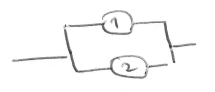
\includegraphics[width=0.3\textwidth]{img/parallel.PNG} \\
	$\mathds{P}[\text{Ausfall des Systems}] = \mathds{P}[A_1\cap A_2] = p_1p_2$
	\item [b)] Reihenschaltung 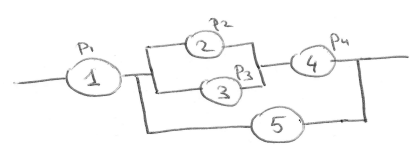
\includegraphics[width=0.3\textwidth]{img/reihe.PNG}\\
	$\mathds{P}[\text{Ausfall des Systems}]= \mathds{P}[\underbrace{A_1 \cup A_2}_{\substack{\text{nicht disj,}\\\text{unabh}}}] = 1-\mathds{P}[(A_1 \cup A_1)^C]\overset{\text{de Morgan}}{=}$\smallskip\\
	$1-\mathds{P}[\underbrace{A_1^C \bigcap A_2^C}_\text{unabh}]$\smallskip\\
	$=1.\mathds{P}[A_1^C]*\mathds{P}[A_2^C]$\smallskip\\
	$=1-(1-p_1)(1-p_2)=p_1+p_2 - p_1p_2$\\

	$\mathds{P}[\text{Ausfall}] = ? $
\end{enumerate}
Ereignis, dass das System ausfällt:\\
A = Ausfall des Systems = $A_1 \cup (A_5\cap (A_4 \cup (A_2 \cap A_3)))$\smallskip\\
$\mathds{P}[A] = ?$\\
$\mathds{P}[\text{2 und 3 fällt aus}] = p_2p_3$\smallskip\\
$\mathds{P}[\text{2,3,4 fällt aus}] = p_2p_3+p_4 -p_2p_3p_4$\smallskip\\
$\mathds{P}[\text{2,3,4,5 fällt aus}] = (p_2p_3+p_4-p_2p_3p_4)p_5$\smallskip\\
$\mathds{P}[A] = p_1 + p_\text{Rest} - p_1p_\text{Rest} =$ ... (Prof sagt trivial) \qed\\\\
\textbf{Definition}: n Ereignisse $A_1, A_2,...,A_n$ sind
\begin{itemize}
	\item paarweise unabhängig, wenn $\mathds{P}[A_i \cap A_j] = \mathds{P}[A_i] * \mathds{P}[A_j] \forall i \neq j$
	\item unabhängig, wenn: $\forall m \in \{2,...,n\} \: \forall 1 \leq i_1 < i_2 <...<i_m\leq n$
	$$\mathds{P}[A_{i1}\cap A_{i2}\cap ... \cap A_{im}] = \mathds{P}[A_{i1}* ... * \mathds{P}[A_{im}]$$
	(D.h. Produktformel gilt für alle Teilfamilien)
\end{itemize} 
\newpage
\textbf{Behauptung}: Blockungslemma\\\\
\textbf{Beispiel}: Seien A,B,C,D,E,F,G unabhängige Ereignisse.
$$(A \Delta C) \cap E^C \cup C, \: B^C\cap F,\: D\cup G \quad \text{unabhängig}$$ 
$$\text{Aber:} \quad A \Delta \mathbf{C} \text{ und } B \cup \mathbf{C} \text{ sind im Allgemeinen abhängig}$$
\textbf{Bemerkungen}:\medskip\\
$\Omega$ und A sind immer unabhängig.\medskip\\
$\mathds{P}[\Omega \cap A] = \mathds{P}[A]=\mathds{P}[\Omega]*\mathds{P}[A]$\medskip\\
$\emptyset$ und A sind immer unabhängig\medskip\\
$\mathds{P}[\emptyset \cap A] = \mathds{P}[\emptyset]=0=\mathds{P}[\emptyset]*\mathds{P}[A]$
\chapter{Satz von Bayes}
\subsubsection{Satz: Formel der totalen Wahrscheinlichkeit}
Sei $\Omega = B_1  \dot{\cup} ... \dot{\cup} B_n $ disjunkte Zerlegung von $\Omega$, d.h. $B_i \cap B_j = \emptyset \: \forall i \neq j$ und $\Omega = B_1 \cup ...\cup B_n$\medskip\\
Sei $\mathds{P}[B_i] \neq 0 \forall i$\medskip\\
Sei A $\subset$ $\Omega$ ein weiteres Ereignis. Dann gilt: 
$$\mathds{P}[A] = \mathds{P}[B_1]*\mathds{P}[A \vert B_1] + \mathds{P}[B_2]*\mathds{P}[A\vert B_2]+...$$\medskip
\textbf{Beweis}: $\mathds{P}[A] = \mathds{P}[A\cap B_1]+\mathds{P}[A \cap B_2] +...= \mathds{P}[B_1]*\mathds{P}[A \vert B_1] + \mathds{P}[B_2]*\mathds{P}[A\vert B_2]+... $\qed\\\\
\textbf{Beispiel}:\medskip\\
1\% der Population ist krank, Rest ist gesund
\begin{tabbing}
	Schnelltest: \= Bei einer kranken Person mit Wahrscheinlichkeit 90\% positiv.\\
	\> Bei einer gesunden Person mit Wahrscheinlichkeit 20\% positiv
\end{tabbing}
A= ''Test ist Positiv''\hspace{1cm} $\mathds{P}[A]= 0,001*0.9+0,99*0,2 = 0,207$\smallskip\\
Lösung mit der Formel\\
$B_1 $ = ''Person krank'' \hspace{1cm} $B_2$ = ''Person gesund''\\
$ \mathds{P}[B_1]=0,01 \Rightarrow  \mathds{P}[B_2] =0,99$\smallskip\\
$\mathds{P}[A \vert B_1] = 0,9 \qquad [\text{nicht } \mathds{P}[A\cap B_1]$\smallskip
$\mathds{P}[A\vert B_2] = 0,2$\smallskip\\
$\mathds{P}[A] = \mathds{P}[B_1]*\mathds{P}[A\vert B_1] + \mathds{P}[B_2]*\mathds{P}[A\vert B_2]$\smallskip\\
$=0,01*0.9+0.99*0,2$\medskip\\
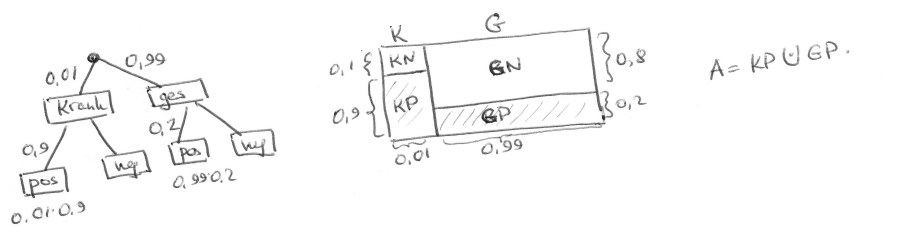
\includegraphics[width=0.9\textwidth]{img/baum.PNG}\\

 \section{Bayes-Formel}
\textbf{Satz 2.2}:\\
Seien A,B $\subset \Omega$ zwei Ereignisse mit $\mathds{P}[A] \neq 0, \mathds{P}[B] \neq 0$. Dann gilt:
$$\mathds{P}[B \vert A] = \dfrac{\mathds{P}[A\vert B] * \mathds{P}[B]}{\mathds{P}[A]}$$
\textbf{Beweis}: Linke Seite = $\mathds{P}[B\vert A] = \dfrac{\mathds{P}[B \cap A]}{\mathds{P}[A]}$\smallskip\\
Rechte Seite = $\dfrac{\mathds{P}[A \vert B] * \mathds{P}[B]}{\mathds{P}[A]} = \dfrac{\mathds{P}[A \cap B]}{\mathds{P}[A]} \qed$\\\\
\textbf{Beispiel 1: (Population Personen: krank und gesund)}\medskip\\
1\% der Population ist krank.
\begin{tabbing}
	Schnelltest: \= Bei einer Kranken Person mit Wahrscheinlichkeit 90\% positiv.\\
	\> Bei einer gesunden Person mit Wahrscheinlichkeit 20\% positiv
\end{tabbing}
Eine gesunde Person wurde positiv getestet.\\
Wahrscheinlichkeit, dass diese Person krank ist?\smallskip
\begin{tabbing}
\textbf{Lösung 1}:\medskip\\
$\Omega$ = Population \hspace{1cm} \= $B_1 = $ ''Person ist krank''\\
\> $B_2 = B_1^C = $ ''Person ist gesund''
\end{tabbing}
A = ''Person wurde positiv getestet''\\
Aufgabenstellung: $\mathds{P}[B_1] = 0,01 \Rightarrow \mathds{P}[B_2] = 1-0,01=0,99$
\begin{enumerate}
	\item $\mathds{P}[A \vert B_1] = 0,9$
	\item $\mathds{P}[A \vert B_2] = 0,2$
\end{enumerate}
$\mathds{P}[B_1\vert A] = ?$\\
Bayes-Formel: $\mathds{P}[B_1 \vert A] \overset{\text{Bayes}}{=} \dfrac{\mathds{P}[A\vert B_1] * \mathds{P}[B_1]}{\mathds{P}[A]} \overset{\text{totale Wkeit}}{=} $\smallskip\\$
\dfrac{\mathds{P}[A \vert B_1]*\mathds{P}[B_1]}{\mathds{P}[A \vert B_1]*\mathds{P}[B_1]+\mathds{P}[A\vert B_2]*\mathds{P}[B_2]} = \dfrac{0,9*0,01}{0,9*0,01+0,2*0,99}= 0,043$\medskip\\
$\mathds{P}[B_2 \vert A] = 1- \mathds{P}[B_1 \vert A ] = 1-0,043$\\\\
\textbf{Lösung 2}:\\ 
$\mathds{P}[A] = 0,01*0,9+0,99*0,2 = 0,207$\medskip\\
$\mathds{P}[\text{krank}\vert \text{positiv getestet}]= \dfrac{0,01*0,9}{0,01*0,9+0,99*0,2} = 0,043$\\\\\\\\
\textbf{Lösung 3}:\\
Laplace-Experiment mit $\Omega = \{\text{KP, KN, GP, GN}\}$\\
P(KP) = 0,9*0,01 \hspace{2cm} P(GP) = 02*0,99\\
P(KN) = 0,1*0,01 \hspace{2cm} P(GN) = 0,8*0,99\smallskip\\
A = ''Person positiv'' = \{KP, GP\}\\
$B_1$ = ''Person krank'' =  \{KP, KN\} 
$$\mathds{P}[B_1\vert A] = \dfrac{\mathds{P}[B_1 \cap A]}{\mathds{P}[A]} = \dfrac{P(\text{KP})}{P(\text{KP})+P(\text{GP})} = ...$$\medskip\\
\textbf{Beispiel 2: (2 Jungen Problem)}\\
Im Nachbarhaus: Familie mit 2 Kindern.\\
Sie beobachten: Im Garten spielt ein Junge.\\
Wkeit, dass das $\underbrace{\text{andere Kind auch ein Junge}}_\text{d.h. beide sind Jungen}$ ist = ?\smallskip\\
\textbf{Lösung}:\\
Grundmenge: $\Omega = \{\text{MM1, MM2, MJ1, MJ2, JM1, JM2, JJ1, JJ2}\}$\\
MM1 = Beides Mädchen, erste Kind im Garten\smallskip\\
B = ''Im Garten spielt ein Junge'' = \{MJ2, JM1, JJ1,JJ2\}\\
A = ''Beide Kinder sind Jungen'' = \{JJ1, JJ2\} \hspace{1cm} $A\cap B = $\{JJ1,JJ2\}\medskip\\
$\mathds{P}[A\vert B] = \dfrac{\mathds{P}[A \cap B]}{\mathds{P}[B]} = \dfrac{2/8}{4/8} = 0.5$\bigskip\\
\textbf{Beispiel 3: (Ziegenproblem)}
\begin{tabbing}
	3 Türen \hspace{1cm} \= Hinter einer Tür $\rightarrow$ Auto\\
	\> Hinter den beiden anderen $\rightarrow$ Ziegen
\end{tabbing}
Sie zeigen auf Tür 1. (Tür 1 bleibt aber geschlossen)\\
Moderator öffnet eine der beiden anderen Türen $\rightarrow$ Ziege.\\
Sie dürfen bei Tür 1 bleiben oder wechseln. Was ist besser?\smallskip\\
Aufgabenstellung ist unvollständig. Wir machen die Annahme: Moderator weiß, wo das Auto steht und will das Auto nicht zeigen.\newpage
\textbf{Lösung}: \\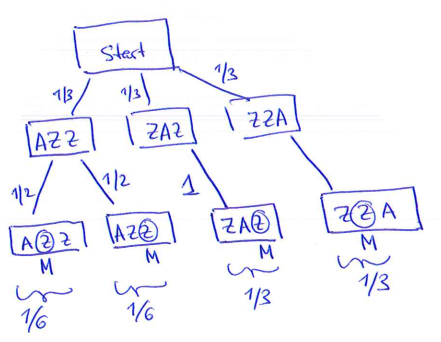
\includegraphics[width=0.6\textwidth]{img/ziege.PNG}\\
$\Omega =$ \{A\textbf{Z}Z, AZ\textbf{Z},ZA\textbf{Z},Z\textbf{Z}A\}\ \hspace{ 1cm} Dick geschrieben: Vom Moderator  gewählt \medskip\\
p(A\textbf{Z}Z) = $\frac{1}{3}*\frac{1}{2}$\smallskip\\
p(AZ\textbf{Z}) = $\frac{1}{3}*\frac{1}{2}$\smallskip\\
p(ZA\textbf{Z}) = $\frac{1}{3}*1$\smallskip\\
p(Z\textbf{Z}A) = $\frac{1}{3}*1$\medskip\\
$\mathds{P}[\text{Auto hinter Tür 1}] $ = p(A\textbf{Z}Z)+p(AZ\textbf{Z}) = $\frac{1}{6}+\frac{1}{6}=\frac{1}{3}$\\
$\mathds{P}[\text{Türwechsel führt zum Erfolg}]$ = p(ZA\textbf{Z})+p(Z\textbf{Z}A) = $\frac{1}{3}+\frac{1}{3}= \frac{2}{3}$\medskip\\
\textbf{Also wechseln!}


\chapter{Zufallsvariablen}
\textbf{Definition}:\\
Eine ZV ist eine Funktion X:$\Omega$ $\rightarrow \mathbb{R}$\smallskip\\\textbf{Beispiel}:\\
2 Würfel. \hspace{1cm}$\Omega = \{(a_1,a_2): a_1,a_2 \in \{1,...,6\}\}$\medskip\\
Erste Augenzahl: $X_1(a_1,a_2)=a_1$\\
Zweite Augenzahl $X_2(a_1,a_2)=a_2$\\
Augensumme: $X(a_1,a_2) = a_1 + a_2 \qquad x = x_1 + x_2$\\
Größe Augenzahl: $y(a_1,a_2)=max(a_1,a_2)$\medskip\\
\textbf{In dieser Vorlesung sei $\Omega$ immer endlich}\medskip\\
\textbf{Definition}:\\
Eine Verteilung einer ZV X ist die Angabe der Werte und der Wahrscheinlichkeiten dieser Werte.\smallskip\\
	Zähldichte von X : $\Omega \rightarrow\mathbb{R}$ ist $P_x:\mathbb{R}\rightarrow[0,1]$\medskip
\begin{center}
	$P_x(t)=\mathds{P}\underbrace{[x = t]}_\text{Er.} = \mathds{P}[\underbrace{\{w \in \Omega:X(\omega)=t\}}_{x^{-1}(t)}]$\medskip\\
\end{center}
	
\textbf{Beispiel}: 2 Würfel. \hspace{1cm} $x(a_1,a_2) = a_1 + a_2$ Augensumme\medskip\\
\begin{tabular}{c|c|c|c|c|c|c|c|c|c|c|c|}
	t&2&3&4&5&6&7&8&9&10&11&12\\\hline
	$\mathds{P}[x=t]$&$\frac{1}{36}$&$\frac{2}{36}$&$\frac{3}{36}$&$\frac{4}{36}$&$\frac{5}{36}$&$\frac{6}{36}$&$\frac{5}{36}$&$\frac{4}{36}$&$\frac{3}{36}$&$\frac{2}{36}$&$\frac{1}{36}$
\end{tabular}\medskip\\
\{x=2\} = \{(1,1)\}\\
\{x=3\}=\{(1,2),(2,1)\}\\
\{x=4\} = \{(1,3),(3,1),(2,2)\}\\
...\medskip\\
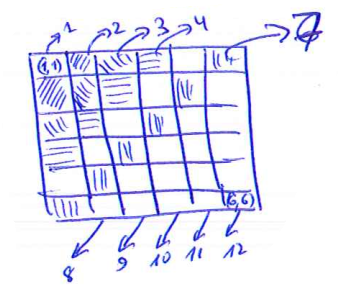
\includegraphics[width=0.4\textwidth]{img/okay.PNG}\\

\begin{math}
P_x(t)=
\begin{cases}
	\dfrac{t-1}{36}&, t \in \{2,...,7\}\medskip\\
	\dfrac{13-t}{36}& , t \in \{7,...,12\}\medskip\\
	0, t \notin \{2,...,12\}
\end{cases}
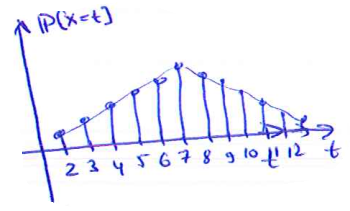
\includegraphics[width=0.4\textwidth]{img/diaa.PNG}\\
\end{math}\begin{floatingfigure}[r]{6cm}
	\mbox{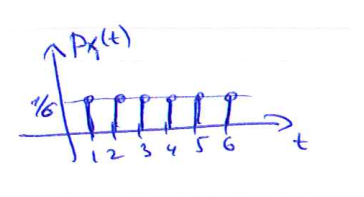
\includegraphics[width=0.4\textwidth]{img/dia.PNG}}
\end{floatingfigure}
Für die erste Augenzahl $x_1(a_1,a_2) = a_1$\medskip\\
\begin{tabular}{c|c|c|c|c|c|c}
	t&1&2&3&4&5&6\\\hline
	$\mathds{P[x_i = t]}$&$\frac{1}{6}$&$\frac{1}{6}$&$\frac{1}{6}$&$\frac{1}{6}$&$\frac{1}{6}$&$\frac{1}{6}$
\end{tabular}\\\\
\textbf{Eigenschaften der Zähldichte: }
\begin{enumerate}
	\item $P_x(t)\in [0,1]$
	\item $\sum_{t\in\mathbb{R}}P_x(t) = 1$
\end{enumerate}
\textbf{Beispiel}: Sei A $\subset$ $\Omega$\\
Indikatorvariable von A:\medskip\\
\begin{math}
\mathds{1}_A(\omega)=
\begin{cases}
1,& \omega \in A\\
0,& \omega \notin A
\end{cases}
\end{math}
\medskip\\
Grafik und Tabelle indikatorvariable\medskip\\
\textbf{Definition}: Sei X ZV mit Verteilung\medskip\\
\begin{tabular}{c|c|c|c|c}
	Werte&$y_1$&$y_2$&$y_3$&...\\\hline
	Wahrscheinlichkeiten&$P_1$&$P_2$&$P_3$&...
\end{tabular} \hspace{1cm}$\smallskip\\\mathds{P}[x = y_i] = p_i$\medskip\\
Erwartungswert von X ist $\mathds{E} X = \sum_i \underbrace{y_i}_\text{Werte} \underbrace{P_i}_\text{Wkeiten}$\medskip\\
\textbf{Beispiel}: 1 Würfel, $x_1$ Augenzahl\\
$\mathds{E}X_1 = 1*\frac{1}{6}+2*\frac{1}{6}+...+6*\frac{1}{6} = 3,5$\\
$\mathds{E}X$ ist \textbf{nicht} der wahrscheinlichste Wert: $\mathds{P} [X=3,5] = 0$\medskip\\
\textbf{Bemerkung:}\\
Betrachte $n=10^6$ Würfe. Augenzahlen: $X_1,X_2,...,X_n$\smallskip\\
Dann gilt $\dfrac{X_1+...+X_n}{n}\approx 3.5$\medskip\\
\textbf{Satz 9.1}$[\text{ alternative Formel für }\mathds{E}X]$\\
Sei $X:\Omega \rightarrow\mathbb{R}$. Dann gilt: 
$$\mathds{E}X = \sum_{\omega \in \Omega} X(\omega)\underbrace{\mathds{P}[\{\omega\}]}_{p(\omega)}$$
\textbf{Beweis}: Seien $y_1,...,y_m$ Werte von X\medskip\\
$A_1 = \{X = y_1\},\dots ,A_m=\{X=y_m\}$\smallskip\\
$A_i = \{\omega \in \Omega:X(\omega)=y_i$s\}\smallskip\\
$\Omega = A_i \dot\cup A_2\dot\cup \dots\dot\cup A_m$ ist disjunkte Zerlegung\smallskip\\
$\mathds{E}X \overset{\text{Def}}{=} \sum_i y_i*p_i = \sum_i y_i \mathds{P}[A_i]$\smallskip\\
$\sum_iy_i\sum_{\omega \in A_i} p(\omega) \overset{w \in A_i}{=}\sum_i \sum_{\omega \in A_i} X(\omega)p(\omega)$ \medskip\\
$	\Rightarrow X(\omega)=y_i$\medskip\\
\textbf{Satz 9.2}. Seien $x,y :\Omega \rightarrow\mathbb{R}$ Zufallsvariablen\smallskip\\
Dann gilt: $\mathds{E}[x+y] = \mathds{E}X+\mathds{E}y$\medskip\\
\textbf{Beweis}: \\
$\mathds{E}[x+y] \underset{9.1}{=} \sum_{\omega \in \Omega}(x+y)(\omega)*p(\omega)=$\smallskip\\
$=\sum_{\omega \in \Omega} (X(\omega)+y(\omega))p(\omega) = \sum_{\omega \in \Omega}X(\omega)*p(\omega)+\sum_{\omega \in \Omega}y(\omega)*p(\omega)\overset{9.1}{=}$\smallskip\\$\mathds{E}X+\mathds{E}y\qed$\medskip\\
\textbf{Bemerkung}: Allgemein: Für ZV $X_1,\dots,X_n : \Omega \rightarrow \mathbb{R}:\mathds{E}[X_1+\dots+X_n] =$\\$ \mathds{E}X_1+\dots+\mathds{E}X_n$\medskip\\
\textbf{Bemerkung}: Sei $X:\Omega \rightarrow \mathbb{R}, a\in \mathbb{R}, \mathds{E}[a*X]=a*\mathds{E}X$\medskip\\
\textbf{Beispiel}: n Würfel. Augenzahlen: $X_1,\dots,X_n$ \hspace{0.2cm} Augensumme: S=$X_1+\dots+X_n$
$$\mathds{E}S=\mathds{E}X_n+\ldots+ \underbrace{\mathds{E}X_n}_{=3,5} = n*3,5$$
\textbf{Beispiel}: Lotto 6 aus 49. (ohne Zurücklegen) Tippe auf \{1,\dots,6\} \\
Sei S die Anzahl der richtig geratenen Zahlen.\medskip\\
Werte von S: 0,1,\dots,6\smallskip\\
$\mathds{P}[S=k] = \dfrac{\binom{6}{k}*\binom{43}{6-k}}{\binom{49}{6}} $ , für k $\in$ \{0,\ldots,6\}\medskip\\
\begin{math}
S = X_1+\dots+X_6, \text{wobei }\medskip\\
X_i = 
\begin{cases}
1,&\text{falls Ball \textbf{i} gezogen wurde}\\
0,&\text{sonst}
\end{cases}\medskip\\
\mathds{E}S\underset{9.2}{=}\mathds{E}X_1+\dots+\mathds{E}X_6
\end{math}\medskip\\
\textbf{Bemerkung}:\medskip\\ $\mathds{E1}_A=$
\begin{tabular}{c|c}
	0&1\\\hline
	$1-\mathds{P}[A]$&$\mathds{P}[A]$
\end{tabular} = $\mathds{P}[A]$\newpage
\begin{math}
\mathds{E}X_i= \mathds{P}[\text{Ball \textbf{i} wurde gezogen}]\medskip\\
= \dfrac{\binom{48}{5}}{\binom{49}{6}}
=\dfrac{\left(\dfrac{48*47*46*45*44}{5!}\right)}{\left(\dfrac{48*47*46*45*44}{6!}\right)} = \dfrac{6!/5!}{49} = \dfrac{6}{49} \quad \forall i \in \{1,\dots,6\}\medskip\\
\mathds{E}S=\mathds{E}X_1+\dots\mathds{E}X_6=6*\dfrac{6}{49}=\dfrac{36}{49}
\end{math}\medskip\\
\textbf{Definition}:\\
Seien $X_1,\dots,X_n : \Omega \rightarrow\mathds{R}$ ZV\\
Sie heißen unabhängig, falls: 
$$\forall y_1,\dots,y_n \in \mathds{R}: \quad \mathds{P}[X_1 = y_1,X_2 =y_2,\dots,X_n=y_n]]$$
$$=\mathds{P}[X_1=y_1]*\dots*\mathds{P}[X_n]=y_n$$
\textbf{Bemerkung}: Sind $X_1,\dots,X_n$ unabhängig, dann gilt sogar:
$$\forall A_1,\dots,A_n \subset \mathds{R}: \mathds{P}[X_1 \in A_1,\dots,X_n \in A_n]$$
$$=\mathds{P}[X_1 \in A_1]*\dots*\mathds{P}[X_n \in A_n]$$\medskip\\
\textbf{Satz 9.3}:\\
Seien $X,Y :\Omega \rightarrow \mathds{R} $ \textbf{unabhängige} Zufallsvariablen\\
Dann gilt: $\mathds{E}[X*Y]= \mathds{E}X*\mathds{E}Y$\medskip\\
\textbf{2 Eigenschaften}:
\begin{enumerate}
	\item $\mathds{E}[x+y] = \mathds{E}x+\mathds{E}y \quad \forall x,y$
	\item $ \mathds{E}[x*y] = \mathds{E}x*\mathds{E}\text{$ y $ } \forall \text{unabh. } x,y$
\end{enumerate}
\textbf{Beweis}:\\
Notation:\\
Werte von X: 
\begin{tabular}{|c|c|c|}
	$x_1$&$x_2$&\dots\\\hline
	$p_1$&$p_2$&\dots
\end{tabular} \\
$\mathds{P}[X=x_i]=p_i$\smallskip\\
Werte von Y: 
\begin{tabular}{|c|c|c|}
	$y_1$&$y_2$&\dots\\\hline
	$q_1$&$q_2$&\dots
\end{tabular}\\
$\mathds{P}[Y=y_j]=p_j$\newpage
Betrachte Ereignisse: $A_{ij}=\{X=x_i, y=y_j\}\smallskip\\=\{\omega \in \Omega : X(\omega)=xi,y(\omega)=y_j\}$\medskip\\
\begin{center}
	\img{0.4}{tab}\\
\end{center}
$\Omega = \underset{i,j}{\dot\cup}A_{ij}$, d.h. $A_{ij}$ bilden disjunkte Zerlegung von $\Omega$\medskip\\
$\mathds{E}[x*y] \underset{9.1}{=} \sum_{\omega\in \Omega} p(\omega)*X(\omega)*Y(\omega)=$\medskip\\
$\sum_{i,j}\sum_{\omega\in A_{ij}} (p(\omega)*X(\omega)Y(\omega)x_iy_j)=$\medskip\\
=$\sum_{i,j}(x_iy_j\sum_{w\in A_{ij}})=\sum_{i,j}x_iy_j\mathds{P}[A_{ij}]$\medskip\\
$\mathds{P}[A_{ij}]=\mathds{P}[X=x_i, Y=y_j] \underset{\text{x,y unabh ZV}}{=} \mathds{P}[X=x_i]*\mathds{P}[Y=y_i]=p_i*q_j$\bigskip\\
$=\sum_{i,j}x_iy_jp_iq_j = \sum_{i,j}(x_ip_i)(y_jq_j)$\medskip\\
$=(\sum_ix_ip_i)(\sum_jy_jq_j) = \mathds{E}X*\mathds{E}Y \qed$\\\\
\textbf{Beispiel}: (zur Unabhängigkeit von Zufallsvariablen)\\
Betrachte n faire Würfel\smallskip\\
$X_i$ ist die Augenzahl, die der i-te Würfel zeigt\smallskip\\
 $\Omega$ = \{($a_1,...,a_n$)\} def $X_i(a_1,...,a_n) = a_i$\medskip\\
 \textbf{Behauptung 1}: Zufallsvariablen $X_1,\dots,X_n$ sind unabhängig\medskip\\
 \textbf{Beweis 1}:\\
 Z.z. $\mathds{P}[X_i = x_1,...,X_n=x_n] = \mathds{P}[X_i=x_i]*\dots\mathds{P}[X_n=x_n]$\medskip\\
$\{X_1 = x_1,\dots X_n = x_n\}=
\begin{cases}
(x_1,\dots,x_n), &\text{falls }\forall i:x_i \in \{1,...,6\}\\
\emptyset, & \text{falls } \exists i : x_i \notin \{1,...,6\}
\end{cases}$\smallskip\\
LS = $
\begin{cases}
\dfrac{1}{6^n},&\text{falls } \forall i: x_i \in \{x_i \in \{1,...,6\}\\
0,&\text{sonst}
\end{cases}$\\\\
RS: $\mathds{P}[X_1=x_1] = ?$\medskip\\
\{$X_1=x_1$\}=$\begin{cases}
\{(x_1,a_2,...,a_n):a_2,...,a_n \in \{1,\dots,6\}\}, &\text{falls }x_1 \in \{1,\dots,6\}\\
\emptyset, & \text{falls } \exists i : x_i \notin \{1,...,6\}
\end{cases}$\medskip\\
$\#\{X_1=x_i\}=\begin{cases}
6^{n-1},&\text{falls }x_1\in \{1,\dots,6\}\\
0,&\text{sonst}
\end{cases}$\medskip\\
$\mathds{P}[X_1=x_1]=\begin{cases}
\dfrac{6^{n-1}}{6^n},&\text{falls }x_1 \in \{1,\dots,6\}\\
0,&\text{sonst}
\end{cases}$\medskip\\
RS=$\begin{cases}
\dfrac{1}{6}*\dfrac{1}{6}*\dots\dfrac{1}{6} = \dfrac{1}{6^n},&\text{falls } \forall A_i : x_i \in \{1,\dots,6\}\\
0, & \exists i:x_i \notin \{1,\dots,6\}
\end{cases}$\\\\
LS = RS $\Rightarrow X_1,\dots,X_n$ unabh. ZV.\\\\
\textbf{Behauptung 2}: Sei S = $X_1 + \dots + X_n$ die Augensumme.\\
Dann sind $X_1$ und S abhängige Zufallsvariablen\medskip\\
\textbf{Beweis}: Z.z. $\exists$ a,b mit $\mathds{P}[X_1=a,S=b] \neq \mathds{P}[X_1=a]*\mathds{P}[S=b]$\\
Wir zeigen das für a =1, b=6*n\medskip\\
\textbf{LS}: $\mathds{P}[\underbrace{X_1=1,S=6n}_\text{Treten nicht gleichzeitig ein}] = 0$\smallskip\\
\textbf{RS}: $\mathds{P}[X_1 = 1] = \dfrac{1}{6}$\\$\mathds{P}[S=6n]=\dfrac{1}{6^n}$\medskip\\
RS = $\dfrac{1}{6}*\dfrac{1}{6^n} \neq 0$\medskip\\
LS $\neq$ RS $\Rightarrow$$X_1,S$ abh. \qed
 

\chapter{Harmonische Reihe}
\section{Harmonische Reihe}
\newcommand{\harmonisch}{\frac{1}{2}+\frac{1}{3}+\frac{1}{4}+\dots}
\textbf{Definition}: Harmonische Zahlen $H_n = 1 + \frac{1}{2}+\frac{1}{3}+\frac{1}{4}+\dots+\frac{1}{n}$\smallskip\\
Harmonische Reihe: $\frac{1}{2}+\frac{1}{3}+\frac{1}{4}+\dots = \underset{n\rightarrow\infty}{\text{lim} }H_n$\medskip\\
\subsection{Satz 10.1}
$\harmonisch = + \infty \qquad H_n = \harmonisch$\medskip\\
d.h. $\forall$ A (egal wie groß) $\exists$ n = n(A) : $H_n \geq A$\smallskip\\
\textbf{Beweis}:\\
\img{0.7}{harm}\\
$H_2 \geq 1 + \frac{1}{2}, H_4 \geq 1+\frac{1}{2}+\frac{1}{2}, H_8 \geq 1+\frac{1}{2}+\frac{1}{2}+\frac{1}{2}$\\
$H_{2^l}\geq 1+\frac{l}{2}$\smallskip\\
$A=7*10^6 \quad 1+\frac{l}{2} \geq A\quad l \geq 2A-2$\\
$H_{2^{1+10^6-2}} \geq 7 * 10^6$
\subsection{Satz 10.2, Euler, 1734}
$\underbrace{\harmonisch+\frac{1}{n}}_{H_n\rightarrow\infty}-\underbrace{\text{log }n}_{\rightarrow\infty} $ konvergiert für n $\rightarrow$ $\infty$ gegen eine Konstante.\medskip\\
\textbf{Bemerkung}: Die Konstante $ \gamma $ := $\underset{n\rightarrow\infty}{\text{0}}(H_n-\text{log } n) = 0,57721\dots $ heißt\\
Euler-Mascheroni-Konstante\smallskip\\
\textbf{Beweis}: $\int_1^n \dfrac{1}{x} dx$ = (log x) $  \big|_1^n$ 1 n = log n - $\underbrace{\text{log 1}}_{0}$ = log n\smallskip\\
\img{0.7}{log}\\
$H_{n-1}  - \text{log } n = $Fläche $S_n$\\
$S_1<S_2<S_3<\dots \qquad$\\$ \text{Außerdem: }S_n \leq 1\: \forall n \in \mathds{N}$
\img{0.3}{1}\\
D.h. $\exists$ lim $S_n$ exisitert und ist $\leq$1 und $\geq$ 0\medskip\\
$H_n - \text{log }n = \underbrace{H_{n-1}-\text{log }n}_{\text{Konv. für n}\rightarrow\infty} + \underbrace{\frac{1}{n}}_0$, also konvertgiert $H_n - \text{log }n$ gegen einem Limes, der zwischen 0 und 1 liegt. \qed\medskip\\
$\harmonisch+\dfrac{1}{n} = \text{log }n + \gamma + \underbrace{\varepsilon_n}_\text{Fehler der Appr.}\text{, wobei }\varepsilon_n \rightarrow 0 \text{ für } n\rightarrow\infty$
\section{Alternierende harm.Reihe}
\newcommand{\altharm}{1-\frac{1}{2}+\frac{1}{3} - \frac{1}{4}+\dots}
Alternierende harm. Reihe: $\altharm = log 2$\medskip\\
\textbf{Beweis}:\\
$S_{2n} = \altharm - \frac{1}{2n}$\smallskip\\
$S_{2n+1}= \altharm -  \frac{1}{2n} + \frac{1}{2n+1}$\medskip\\
$S_{2n} = \altharm - \frac{1}{2n} = H_{2n}-2(\frac{1}{2}+\frac{1}{4}+\dots+\frac{1}{2n})$\smallskip\\
$=H_{2n} - (1+\frac{1}{2}+\frac{1}{3}+\dots+\frac{1}{n})=H_{2n}-H_n = $\smallskip\\
$\underset{\text{Kor.}}{=} (\text{log }2n+ \gamma + \varepsilon_{2n}) - (\text{log }n + \gamma + \varepsilon_n)$\smallskip\\
$=\text{log }2n - \text{log }n + \varepsilon_{2n}-\varepsilon_n$\smallskip\\
$=\text{log }2 + \underbrace{\varepsilon_{2n}}_0-\underbrace{\varepsilon_n}_0\quad$
$\underset{n\rightarrow\infty}{\rightarrow} log 2$\medskip\\

\textbf{Aufgabe}: Schnecke und Auto\\
$1+\dfrac{1}{2}+\dfrac{1}{3}+\dots = \infty$\medskip\\
\imgHere{schneckeUndAuto}\\
\textbf{Zeige}: Schnecke überholt das Auto in endlicher Zeit\\
$\altharm$ = log 2\smallskip\\
$\underbrace{1+\frac{1}{3}-\frac{1}{2}}+\underbrace{\frac{1}{5}+\frac{1}{7}-\frac{1}{4}}+\underbrace{\frac{1}{9}+\frac{1}{11}-\frac{1}{6}}\dots = \frac{3}{2}\text{ log 2}$\medskip\\
Reihe $\sum_{n=1}^{\infty}$ heißt absolut konvergent, wenn $\sum_{n=1}^\infty |a_n|<\infty$\\
\textbf{Beispiel}:$\altharm $ ist konvergent aber nicht absolut konvergent.\medskip\\
\textbf{Satz}: In einer absolut konvergenten Reihe kann man die Terme umordnen, ohne dass sich die Summe ändert.\\
\textbf{Riemann'scher Umordnungssatz}: $\forall a \in \mathbb{R}$ gibt es eine Umordnung der Reihe $\altharm$, die gegen a konvergiert.\medskip\\
\textbf{Beweis}: Sei $a\geq 0$\\
Ungerade Terme: 1, $\frac{1}{3}, \frac{1}{5},\dots \quad 1 + \frac{1}{3}+\frac{1}{5}\dots = \infty$\medskip\\
Gerade Terme: $\frac{1}{2},\frac{1}{4},\dots \quad \frac{1}{2}+\frac{1}{4}+\dots = \infty$\medskip\\
Nehme ungerade Terme bis die Summe $\geq$ a wird: 
$$1+\dfrac{1}{3}+\dfrac{1}{5}+\dots+\frac{1}{n_1}\geq a$$
Ziehe gerade Terme abm bis die Summe $\leq$ a wird
$$1+\dfrac{1}{3}+\dfrac{1}{5}+\dots+\frac{1}{n_1}-\dfrac{1}{2}-\dfrac{1}{4}-\dots-\frac{1}{m_1}\leq a$$
Addiere ungerade Terme bis die Summe wieder $\geq$ a wird
$$1+\dfrac{1}{3}+\dfrac{1}{5}+\dots+\frac{1}{n_1}-\dfrac{1}{2}-\dfrac{1}{4}-\dots-\frac{1}{m_1}+\dfrac{1}{n_1+2}+\dfrac{1}{n_1+4}+\dots +\dfrac{1}{n_2}\geq a$$usw. \qed\medskip\\
\textbf{Bemerkung} Über EWert von ZV mit abzählbar $\infty$-vielen Werten\smallskip\\
Betrachte ZV X: \hspace{1cm} Werte: \begin{tabular}{c|c|c|c}
	$x_1$&$x_2$&$x_3$&\dots\\\hline
	$p_1$&$p_2$&$p_3$&\dots
\end{tabular}\medskip\\
$\mathds{E}X=\sum_{i=1}^\infty x_ip_i ?$ \\
\textbf{Problem:} Keine ''kanonische'' Reihenfolge der Werte $x_i$ Wenn $\sum_{i=1}^\infty$ nicht \textbf{absolut} konv. $\Rightarrow$kann sich das Ergebnis durch Umordnung ändern\medskip\\
\textbf{Definition}: Sei X ZV wie oben Def.
$$S_+ = \sum_{i:x_i \geq 0}x_ip_i,\quad S_ = \sum_{i:x_i < 0}|x_i|p_i$$
\textbf{Fälle}:$
\begin{cases}
	 \mathds{E}X\overset{\text{def}}{=}\sum_{i=1}^\infty x_ip_i = S_+-S_-,  &\text{falls }S_+ < \infty, s_- < \infty\\
	 \mathds{E}X\overset{\text{def}}{=}+\infty,&\text{falls } S_+=\infty, s_- < \infty\\
	\mathds{E}X \overset{\text{def}}{=}-\infty,&\text{falls } S_+ < \infty, S_- = \infty\\
\mathds{E}X \text{nicht definiert }, & \text{falls } S_+ = \infty, S_-=\infty
\end{cases}$

\chapter{Diskrete Verteilungen}
\section{Uniforme Verteilungen}
\textbf{Definition}:\\
ZV X heißt uniform, falls verteilt auf der Menge \{$x_1$,\dots$x_n$\} ($x_i \in \mathds{R}$), falls: 
$$\mathds{P}[X=x_i] = \dfrac{1}{n} \forall i = 1,\dots,n$$
\textbf{Bemerkung}: $\mathds{E}X= x_1*\dfrac{1}{n}+x_2\dfrac{1}{n}+\dots + x_n *\dfrac{1}{n} = \dfrac{x_1+\dots+x_n}{n} \quad [\text{arithmetisches Mittel}]$\medskip\\
\textbf{Beispiel}:\\
Sei X uniform verteilt auf \{1,2,\dots,n\} $\mathds{E}X=\dfrac{1+2+\dots+n}{n}=$\smallskip\\
1+2+\dots + n = $\dfrac{n(n+1)/2}{n}=\dfrac{n+1}{2}$ \\
\imgHere{Treppe}\\
$=\dfrac{n^2}{n}+\dfrac{n}{2}=\dfrac{n(n+1)}{2}$\medskip\\
\begin{math}
1 + 3 + 5 + 7 + \dots + (2n-1)\\
n = 1: 1\\
n = 2: 1+3=4\\
n = 3: 1 + 3 + 5 = 9\\
\dots
\end{math}
Vermutung: $1 + 3 + 5 + \dots (2n-1) = n^2$\\
Proof by picture:\\
\imgHere{proofByPicture}
\section{Binomialverteilung}
Ein Bernoulli-Exp: Zwei Ausgänge $\underbrace{\text{Erfolg}}_p$ (oder 1) und $\underbrace{\text{Misserfolg}}_{1-p}$ (0)\medskip\\
\textbf{Definition}:\\
ZV X heißt Bernoulli-verteilt, falls 
$$\mathds{P}[x=1]=p,\mathds{P}[x=0]=1-p$$
Bez: $x^\sim$ Bern(p)\\
$\mathds{E}X=1*p+0*(1-p)=p$\smallskip\\
Nn betrachte n unabh. Bern-Exp. Grundmenge: $\Omega =\{(0,1)^n:a_i \in \{0,1\}\}$\smallskip\\
$\mathds{P}[(0,0,1,0,1,1)]=(1-p)*(1-p)*p*(1-p)*p*p = p^3(1-p)^3$\smallskip\\
$\mathds{P}[(A_1,\dots,a_n)]= p^k(1-p)^{a-k}$, wobei K $= a_1,+\dots,+a_n $(Anzahl Erfolge)\medskip\\
Für $p=\frac{1}{2} \Rightarrow$ LaPlace-Experiment\\
Für $p \neq \frac{1}{2} \Rightarrow$ kein LaPlace-Experiment
\subsubsection{Satz 11.1}
Sei X die Anzahl der Erfolge in einem n-fachen Bernoulli-Experiment.\\
Dann gilt: $\mathds{P}[x=k]= \binom{n}{k}*p^k(1-p)^{n-k} \quad k = 0,1,\dots,n$\medskip\\
\textbf{Beispiel}:\\
$n=4, k=2$\smallskip\\
\begin{tabular}{ll}
$	\mathds{P}[(1,1,0,0)] = p^2*(1-p)^2$ & (1,0,1,0)\\
$\mathds{P}[(0,1,1,0)= p^2(1-p)^2$ & (1,0,0,1)\\
	&(0,0,1,1) 
\end{tabular}\smallskip\\
Alle 6 Ausgänge haben Wkeit $p^2(1-p)^2$\medskip\\
\textbf{Definition}:\\
ZV X wie oben heißt binomialverteilt mit Param n und p\\
Bez: $x^\sim$Bin(n,p)\smallskip\\
\textbf{Bemerkung}: $\sum_{k=0}^n\mathds{P}[x=k]=\sum_{k=0}^n\binom{n}{k}p^k(1-p)^{n-k}\overset{Bin. Formel}{=}(p+1-p)^n = 1^n=1$\medskip\\
\subsubsection{Satz 11.2}
Sei $X^\sim$Bin(n,p)\\
Dann gilt $\mathds{E}X=n*p$\medskip\\
\textbf{Beweis}:\\Sei 
$x_i = \begin{cases}
1&,\text{falls im i-ten Experiment Erfolg eintritt}\\
0&,\text{sonst}
\end{cases}$\smallskip\\
$\underbrace{x}_{\substack{\text{Anzahl d. Erfolge}\\\text{ in Exp. 1,...,i}}} = x_1 + x_2 + \dots + x_n$\smallskip\\
$\mathds{E}x = \mathds{E}[x_1+\dots+x_n]=\overbrace{\mathds{E}x_1}^p+\dots + \overbrace{\mathds{E}x_n}^p = n*p$\smallskip\\
Dann $\mathds{E}x_i = 1*p + 0*(1-p)=p$ \qed\medskip\\
\textbf{Beispiel}: Werfe faire Münze n Mal\\
$\mathds{P}[\text{die Münze zeigt k mal Kopf}]=\binom{n}{k}*(\frac{1}{2}^k)*(\frac{1}{2}^{n-k}) = \dfrac{\binom{n}{k}}{2^n}$\smallskip\\
\textbf{Beispiel}: Werfe fairen Würfel n Mal\\
$\mathds{P}[\text{k Sechsen}]=\binom{n}{k}*(\frac{1}{6})^k*(\frac{5}{6})^{n-k}$\smallskip\\
\textbf{Beispiel}: Betrachte Urne mit 10 roten und 20 schwarzen Bällen. \\Wir ziehen 15 Bälle \textbf{mit} Zurücklegen.\\
Bestimme Wkeit, dass bei 8 Ziehungen roter Ball gezogen wurde\smallskip\\
n = 15, p = $\frac{1}{3}$\\
Gesuchte Wkeit ist: $\binom{15}{8}*(\frac{1}{3})^8*(\frac{2}{3}^7)$
\chapter{Geometrische Verteilung}
Betrachte unendl. Folge von unabh. Bernoulli-Exp. mit Erfolgswkeit p $\in(0,1]$\\
$\Omega = \{0,1\}^\infty= \{(a_1,a_2,\dots):a_i \in \{0,1\}\}$\smallskip\\
\begin{tabbing}
	Zeitpunkt des ersten Erfolges: \= T : $\Omega \rightarrow\mathds{R}$\\
	\> T$(a_1,a_2,\dots)=\text{min}\{n \in \mathds{N}:a_n = 1\}$
\end{tabbing}
Z.b. T($\underbrace{0}_{a_1}, \underbrace{0}_{a_2} , \underbrace{0}_{a_3}, \underbrace{0}_{a_4}, \underbrace{1}_{a_5},\dots)$ = 5\\
Vert von T? Werte von T:1,2,3,\dots,$\infty$\medskip\\
\subsubsection{Satz 11.3}
$\forall k \in \{1,2,\dots\}:\mathds{P}[T=k]=p(1-p)^{k-1}$\smallskip\\
\textbf{Definition}:T heißt geometrisch Verteilt mit Parameter p. Bez: T $\sim $Geo(p)\smallskip\\
\textbf{Beweis}: Damit T = k ist, muss die Serie wie folgt aussehen: 
$$\underbrace{0,0,\dots,0}_{k-1 \text{ Misserfolge}},\underbrace{1}_\text{Erfolg},\dots$$
Sei $x_i$ das Ergebnis des i-ten Experiments.\\
$x_i$ ist ZV mit $\mathds{P}[x_i=1]=p, \mathds{P}[x_i=0]=1-p. \quad x_1,x_2 $ sind unabh. ZV\smallskip\\
$\mathds{P}[T=k] = \mathds{P}[x_1=0,x_2=0,\dots,x_{k-1}=0,x_n=1] $
$\underset{x_1,\dots,x_n \text{ unabh Zv}}{=} $\\$\mathds{P}[x_i = 0]* \dots * \mathds{P}[x_{k-1}=0]*\mathds{P}[x_k=1]$\medskip\\
$=\underbrace{(1-p)*\dots*(1-p)}_{k-1}P=p(1-p)^{k-1}\qed$\medskip\\
\textbf{Beispiel}: Werfen eine fairen Münze bis zum ersten Mal Kopf.\\
T=Anzahl der Würfe. $\mathds{P}[T-k] \underset{p=\frac{1}{2}}{=}\frac{1}{2}*\frac{1}{2^{k-1}}=\frac{1}{2^k},k=1,2,\dots$\medskip\\
\textbf{Bemerkung}: $\sum_{k=1}^\infty \frac{1}{2^k}=\frac{1}{2}+\frac{1}{4}+\frac{1}{8}+\dots = 1$\smallskip\\
\imgHere{GlasWasser}\medskip\\
\subsubsection{Exkurs über die geometrische Reihe}
\textbf{Aufgabe}: Berechne $1+q+q^2+q^3+\dots+q^n$\smallskip\\
Sei A = $1+q+q^2+q^3+\dots+q^n$\\
Betrachte: q*A = $1+q+q^2+q^3+\dots+q^n+q1 {n+1}$\smallskip\\
Abziehen:\\
$A-qA = 1-q^{n+1}$\\
$A(1-q)=1-q^{n-1}$\smallskip\\
$A \underset{q\neq 1}{=} \dfrac{1-q^{n-1}}{1-q}=\dfrac{q^{n+1}-1}{q-1} \quad \text{Für q=1}: A=n+1 \qed$\smallskip\\
\textbf{Aufgabe}: Berechne $1+q+q^2+q^3+\dots$\\
\textbf{Lösung}: Sei S = $1+q+^2+\dots$\medskip\\
$S \underset{\text{def}}{=} \underset{n\rightarrow\infty}{\text{lim}}(1+q+q^2+\dots+q^n)= \underset{n\rightarrow\infty}{\text{lim}} \dfrac{q^{n+1}-1}{q-1} = \begin{cases}
\dfrac{1}{1-q}&,\text{falls }|q|<1\\
+\infty &,\text{falls }q>1\\
\text{exisitert nicht}&,\text{falls }q\leq -1
\end{cases}\medskip\\$\medskip\\
Denn $\underset{n\rightarrow\infty}{\text{lim}}q^{n+1}?\underset{n\rightarrow\infty}{\text{lim}}q^n=
\begin{cases}
0 &,\text{falls } |q|<1\quad (\dfrac{1}{2})^n \rightarrow 0\\
1&,\text{falls } q = 1\\
+\infty &, \text{falls }q >1 \quad 2^n \rightarrow+\infty\\
\text{existiert nicht}&,\text{falls }q \leq -1\quad \text{divergiert}
\end{cases}$\smallskip\\
Für q = 1: S = 1+1+1+\dots = $\infty$\medskip\\
\textbf{Bemerkung}: Vorsicht mit der Reihe S=1-1+1-1+1-1+\dots Sie divergiert.
\subsubsection{Geometrische Verteilung}
$\sum_{k=1}^\infty \mathds{P}[T=k]=\sum_{k=1}^\infty p\underbrace{(1-p)}_q^{k-1} = p\underbrace{(1+q+q^2+\dots)}_\text{gelöst} = p*\dfrac{1}{1-q}=\dfrac{p}{p}=1$
\subsubsection{Satz 11.4}
Sei T $\sim$ Geo (p) \\
$\mathds{E}T=\dfrac{1}{p}$ \\
\textbf{Bemerkung}:\\
$p\downarrow0 \Rightarrow \mathds{E}T \rightarrow\infty $\\
$p=1 \Rightarrow\mathds{E}T=1$\medskip\\
\textbf{Beweis}: \\
$\mathds{E}T=\sum_{k=1}^\infty k*\mathds{P}[T=k]=\sum_{k=1}^\infty k*p(1-p)^{k-1}=p\sum_{k=1}^\infty k*q^{k-1}$\medskip\\
$\sum_{k=1}^\infty kq^{k-1}=1+2q+3q^2+4q^3+5q^4+\dots$ (Entsteht durch Ableiten von $1+q+q^2+\dots = \dfrac{1}{1-q} $)\smallskip\\
= $( 1+q+q^2+q^3+\dots)'=-\dfrac{1}{(1-q)^2}$\smallskip\\
= $(\frac{1}{1-q})'=-1\dfrac{1}{(1-q)^2}*(1-q)'=\dfrac{1}{(1-q)^2} \quad (\frac{1}{x})' =-\frac{1}{x^2}$\medskip\\
$\mathds{E}T = p*\dfrac{1}{(1-q)^2} = \frac{p}{p^2}=\frac{1}{p} \qed$\medskip\\
\textbf{Beispiel}:\\
Werfe eine faire Münze, sie zum ersten mal Kopf zeigt. Wkeit, dass die Anzahl der Würfe gerade ist.\medskip\\
\textbf{Lösung}: $T \sim $ Geo($\frac{1}{2}$) \\
$\mathds{P}[T\in \{2,4,6,\dots\}] = \mathds{P}[T=2]+\mathds{P}[T=4] + \dots$\smallskip\\
$=\dfrac{1}{2^2}+\dfrac{1}{2^4}+\dfrac{1}{2^6}+\dots$\smallskip\\
$=\dfrac{1}{1- 1/4}-1= \dfrac{4}{3}-1=\dfrac{1}{3}$\bigskip\\
\textbf{Beispiel}: Würfeln mit einem fairen Würfel bis zu ersten 6. Erwartete Anzahl der Würfe?\medskip\\
\textbf{Lösung}:  Erfolg = 6 \hspace{1cm} $p=\frac{1}{6} \mathds{E}T=\dfrac{1}{1/6}=6$\medskip\\
\textbf{Beispiel Sammler-Problem}:\\
Jede Packung enthält ein Bild. Es gibt n mögl. Bilder, alle gleichwahrscheinlich.\\
Erwartete Anzahl an Packungen, die man kaufen muss, um alle Bilder zu sammeln. \medskip\\
\textbf{Lösung}:\\
\textbf{Wartezeit}: $S_n = T_1+T_2+T_3+\dots+T_n$\smallskip\\
mit $T_1 =1, T_2 \sim \text{Geo}(\dfrac{n-1}{n}),T_3\sim \text{Geo}(\dfrac{n-2}{n}),\dots,T_n\sim \text{Geo}(\dfrac{1}{n})$\medskip\\
Hier ist $T_i$ die Wartezeit auf ein noch nie gesehenes Bild nachdem i-1 Bilder gesammelt wurden.\smallskip\\
$T_i \sim \text{Geo}(\dfrac{n-i+1}{n})$\smallskip\\
\begin{tabbing}
	$\mathds{E}S_n = \mathds{E}[T_1+\dots+T_n]$\=$ = \mathds{E}T_1+\mathds{E}T_2+\dots+\mathds{E}T_n$\\
	\> $= \underbrace{1}_{\dfrac{n}{n}}+\dfrac{n}{n-1}+\dfrac{n}{n-2}+\dots+\dfrac{n}{1}$\\
	\>$=n(\dfrac{1}{n}+\dfrac{1}{n-1}+\dots+1)= n(1+\dfrac{1}{2}+\dfrac{1}{3}+\dots+\dfrac{1}{n}) \qed$
\end{tabbing}
Für $n \rightarrow\infty \quad \dfrac{\mathds{E}S_n}{n \text{log}n}\rightarrow1$
\subsubsection{Satz 11.5: Vergessenseigenschaft der Geo-Vert}
$\mathds{P}[T>n+k\vert T>n]=\mathds{P}[T>k] \quad \forall n,k \in \mathds{N}, T \sim \text{Geo}(p)$\\
$[\text{auch:}\mathds{P}[T>n+k\vert T>n]=\mathds{P}[T>k]$\medskip\\
\textbf{Beweis}: $\mathds{P}[T>k] = \mathds{P}[\text{Versuche } 1,2,\dots,k \text{ sind Misserfolge}]=(1-p)^k$\smallskip\\
$\mathds{P}[T>n+k\vert T>n]\underset{\text{def}}{=} \dfrac{\mathds{P}[T>n+k, T>n]}{\mathds{P}[T>n]} = \dfrac{\mathds{P}[T>n+k]}{\mathds{P[T>n]}}$\\$=\dfrac{(1-p)^{1-k}}{(1-p)^n}=(1-p)^k$



\chapter{Poisson Verteilung}
\section{Exkurs über die Zahl e}
\textbf{Beispiel}: Preis steigt jeden Tag um 1 \%\\ Am Anfang: 1 Euro\\ Preis nach 100 Tagen = ?\smallskip\\
\textbf{Lösung}:\\
x $\rightarrowtail x + \dfrac{x}{100}$\smallskip\\
\begin{tabular}{c|c|c|c|c}
	Tag 0&Tag 1&Tag 2&\dots&Tag 100\\\hline
\rule{0pt}{4ex}    	1 &$1+\dfrac{1}{100}$&$\left(1+\dfrac{1}{100}\right)^2$&\dots&$\left(1+\dfrac{1}{100}\right)^{100}$
\end{tabular} $ \approx $ 2,7\medskip\\
Betrachte $a_n = (1+\dfrac{1}{n})^n$\\
n = 100: \textbf{2,7}04813\dots\\
n = 10000: \textbf{2,7181}459 \dots\\\dots\medskip\\
\textbf{Definition}: e = $\underset{n\rightarrow\infty}{\text{lim}} = (1+\dfrac{1}{n})^n = 2,7182818\dots$\medskip\\
$1 + \dfrac{1}{n}\underset{n \rightarrow \infty}{\rightarrow}1 \quad \text{Unbestimmtheit } 1^\infty$\medskip\\
\textbf{Formel 1}:\\
$(1 + \dfrac{x}{n})^n=\left(\left(1+\dfrac{x}{n}\right)^{\dfrac{n}{x}}\right)^x = \left(\left(1+\dfrac{1}{m}\right)^m\right)^x\underset{n \rightarrow\infty}{\rightarrow}e^x\quad x = \text{konst}, n \rightarrow \infty$\medskip\\
\textbf{Beispiel}: $(1+\dfrac{1}{n})^n = (1+\dfrac{1}{n^2})^{n^2*\dfrac{1}{n}}= ((1+\dfrac{1}{n^2})^{n^2})^{\dfrac{1}{n}} \underset{n\rightarrow\infty}{\rightarrow} e^0 = 1$\medskip\\
\textbf{Formel 2}:\\
$e^x = \sum_{k=0}^{\infty}\dfrac{x^k}{k!}=1+x+\dfrac{x^2}{2!}+\dfrac{x^3}{3!}+\dots$\smallskip\\
\textbf{Beweis}:
\begin{enumerate}
	\item $(a+\dfrac{x}{n})^n \rightarrow e^x$
	\item $(1+\dfrac{x}{n})^n = \sum_{k=0}^n \binom{n}{k}(\dfrac{x}{n})^k*1 {n-k}$\smallskip\\$=\sum_{k=0}^n \dfrac{n(n-1)*\dots*(n-k+1)}{k!}*\dfrac{x^k}{n^k}$\smallskip\\
	$= \sum_{k=0}^n \dfrac{x^k}{k!}\underbrace{\dfrac{n(n-1)*\dots*(n-k+1)}{n^k}}_{1} \underset{n \rightarrow \infty}{\rightarrow}\sum_{k=0}^\infty\dfrac{x^k}{k!}$\medskip\\
	$\dfrac{n(n-1)\dots(n-k+1)}{n^k}=\underbrace{\dfrac{1}{n}}_1*\underbrace{\dfrac{n-1}{n}}_1 \dots *\underbrace{\dfrac{n-k+1}{n}}_1 \underset{n\rightarrow\infty}{\rightarrow}1$
\end{enumerate}
\textbf{Beispiel}: x = 1
$$e = 1+1+\dfrac{1}{2!}+\dfrac{1}{3!}+\dots$$
\section{Poisson Verteilung}
\newcommand{\ntoinf}{\underset{n\rightarrow\infty}{\rightarrow}}
Sehr viele Bern.-Exp: $n\rightarrow \infty$\\
Sehr kleine Erfolgswahrscheinlichkeit: $p=\dfrac{\lambda}{n} \quad \lambda =\text{ const.}\quad \lambda >0$\smallskip\\
Die Anzahl der Erfolge ist ZV $S_n \sim$ Bin$(n,\dfrac{\lambda}{n}) \quad \mathds{E}S_n = n*\dfrac{\lambda}{n}=\lambda$\medskip\\
\textbf{Beispiel}: Wkeit, dass es keinen Erfolg gibt: $\mathds{P}[S_n = 0] = (1-\dfrac{\lambda}{n})*(1-\dfrac{\lambda}{n})*\dots*(1-\dfrac{\lambda}{n}) = (1-\dfrac{\lambda}{n})^n \ntoinf e^{-\lambda} \quad [\text{Formel 1}] x = -\lambda$\medskip\\
$\underset{\text{Wkeit k Erfolge}}{\mathds{P}[S_n=k]} = \binom{n}{k}*p^k(1-p)^{n-k} = \binom{n}{k}*(\dfrac{\lambda}{n})^k(1-\dfrac{\lambda}{n})^{n-k} = \underbrace{(1-\dfrac{\lambda}{n})^n}_{e^{-\lambda}}*\underbrace{(1-\dfrac{\lambda}{n})^{-k}}_1 *\lambda^k$\medskip\\
$*\dfrac{n(n-1)\dots(n-k+1)}{k!n^k}\ntoinf e^{-\lambda}*1*\lambda^k*1*\dfrac{1}{k!}$\smallskip\\
$=e^{-\lambda}\dfrac{\lambda^k}{k!}, \quad k = 0,1,2,\dots$\medskip\\
\textbf{Definition}: ZV X heißt Poissonverteilt mit Parameter $\lambda >0$, falls 
$$\mathds{P}[x=k]=e^{-\lambda}*\dfrac{\lambda^k}{k!}, \quad k=0,1,2,\dots$$
\textbf{Bemerkung}:
$$\sum_{k=0}^\infty \mathds{P}[x=k]=\sum_{k=0}^\infty e^{-\lambda}\dfrac{\lambda^k}{k!}=e^{-\lambda} \sum_{k=0}^\infty \dfrac{\lambda^k}{k!}=e^{-\lambda}*e^\lambda = 1$$
\subsection{Satz 11.6: Poisson-Grenzwertsatz}
Sei $S_n \sim$Bin($n\dfrac{\lambda}{n}$), $\lambda >0$ konstant.\smallskip\\
Dann gilt
$$\underset{n\rightarrow\infty}{\text{lim}}\mathds{P}[S_n=k] = \dfrac{e^{-\lambda}\lambda^k}{k!}\quad \forall k = 0,1,2,\dots$$
\begin{tabbing}
	\textbf{Beispiel}:\= 100 Personen\hspace{1cm}A=''mind. eine Person hat heute Geburtstag''\\$\mathds{P}[A] = ?$
\end{tabbing}
\textbf{Lösung 1 (Exakt)}: n=100, Bern-Exp\\
Erfolge im Exp i $ \Leftrightarrow $ Person i hat heute Geburtstag\\Erfolgswkeit p = $\dfrac{1}{365}$\smallskip\\
$A^C$ ''keine Person hat heute Geburtstag''\\
$\mathds{P}[A^C] = \binom{n}{0}p^0(1-p)^n=(1-p)^n $\smallskip\\
$\mathds{P}[A]=1-\mathds{P}[A^C]=1-(1-p)^n=1-\left(1-\dfrac{1}{365}\right)^{100} = 0,2399$\medskip\\
\textbf{Lösung 2 (Approximation)}: Anzahl d. Personen die heute Geburtstag haben: $S_n \sim $ Bin($\underbrace{100}_n,\underbrace{\dfrac{1}{365}}_p$)
$$\mathds{P}[A]=\mathds{P}[S_n \geq 1] = 1-\mathds{P}[S_n=0]$$
$$S_n \sim \text{Bin}(\underbrace{100}_n,\underbrace{\dfrac{1}{365}}_{\dfrac{\lambda}{n}})\approx \text{Poi}(\underbrace{\dfrac{100}{365}}_\lambda)$$
$\mathds{P}[A] = 1-\mathds{P}[S_n=0] \approx 1 - \mathds{P}[\text{Poi}\left(\dfrac{100}{365}\right)=0]$\smallskip\\
$=1-e^{-\lambda}\dfrac{\lambda^0}{0!}=1-e^{-\lambda}=1-e^{-\dfrac{100}{365}} = 0,2396$\medskip\\
\textbf{Beispiel}: 96 \% Prozent der Fluggäste erscheinen. 75 Flugkarten für 73 Plätze verkauft.\medskip\\
$\mathds{P}[\underbrace{\text{alle Fluggäste bekommen Platz}}_A] = ?$\medskip\\
\textbf{Lösung 1 (Exakt)} Die Anzahl der Gäste, die erscheinen: ZV $T_n \sim $Bin(75,096)\smallskip\\
$\mathds{P}[A] = \mathds{P}[T_n\leq 73] = 1-\mathds{P}[T_n \geq 74]=1-\mathds{P}[T_n = 74]-\mathds{P}[T_n=75]$\smallskip\\
=$1-\binom{75}{74}p^{74}(1-p)^1\binom{75}{75}*p^{75}(1-p)^0$\smallskip\\
$\underset{p = 0,96}{=} 1- 75*0,96^{74}*0,04-0,96^{75}=0,8069\dots$\medskip\\
\textbf{Lösung 2 (Approx)}: $T_n \sim \text{Bin}(\underbrace{75}_n,\underbrace{0,96}_{\dfrac{\lambda}{n}})  \approx \text{Poi}(75*0,96)$\smallskip\\
Falsch, da 0,96 nicht klein ist\medskip\\
Betrachte Gäste, die nicht erschienen sind: Anzahl:\smallskip\\
$S_n \sim \text{Bin}(\underbrace{75}_\text{groß},\underbrace{0,04}_\text{klein}) \approx \text{Poi}(\underbrace{75*0,04}_\lambda)$\medskip\\
$\mathds{P}[A] = \mathds{P}[S_n \geq 2] = 1- \mathds{P}[S_n = 0] - \mathds{P}[S_n = 1] \approx 1- e ^{-\lambda}\dfrac{\lambda^0}{0!}-e ^{-\lambda}\dfrac{\lambda^1}{1!}$\smallskip\\
$=1-e^{-75*0,04}-e^{-75*0,04}*75*0,04=0,8008$
\subsection{Satz 11.7}
Sei $x \sim $ Poi($ \lambda $) ($\lambda >0$). Dann gilt $\mathds{E}x= \lambda$\medskip\\
\textbf{Beweis}:\\
\begin{math}
\mathds{E}x = \sum_{k=0}^\infty k \mathds{P}[x=k]= \sum_{k=0}^\infty k *e^{-\lambda}\dfrac{\lambda^k}{k!}\smallskip\\
=\sum_{k=1}^\infty ke^{-\lambda}\dfrac{\lambda^k}{k!} = e^{-\lambda}\sum_{k=1}^\infty \dfrac{\lambda^k}{(k-1)!}\smallskip\\
=e^{-\lambda}\lambda\sum_{k=1}^\infty \dfrac{\lambda^{k-1}}{(k-1)!}\overset{\text{l=k-1}}{=} e^{-\lambda}\lambda\sum_{l=0}^{\infty}\dfrac{\lambda^l}{l!}=e^{-\lambda} \lambda e^\lambda = \lambda
\end{math}\medskip\\
\begin{tabbing}
	\textbf{Faltungsformel}: \= Seien x,y unabh. ZV mit Werten in \{0,1,2,\dots\}\\
	\> Vert von x,y seien gegeben\\
	\> Vert von x+ ?
\end{tabbing} 
\textbf{Lösung} Werte von x+y sind in \{0,1,\dots\}\smallskip\\
Für $n \in \{0,1,2,\dots\} \quad \mathds{P}[x+y=n]=\sum_{k=0}^n\mathds{P}[x=k,y=n-k] \overset{x,y \text{unabh}}{=}\sum_{k=0}^n\mathds{P}[x=k]*\mathds{P}[y=n-k]$\smallskip\\
x = $k \in \{1,2,\dots\} \quad y = n-k$\medskip\\
\textbf{Beispiel}: $x \sim \text{Bin}(m_1,p) \quad y \sim \text{Bin}(m_2,p), \text{unabh.}$\smallskip\\
$x+y \sim \text{Bin}(m_1+m_2,p)$
\chapter{Varianz und Kovarianz}
\textbf{Definition}: Sei X eine ZV. Varianz von X: \hspace{1cm} Var X=$\mathds{E}[(X-\mathds{E}X)^2]$\medskip\\
\textbf{Beispiel}: 
Sei X uniform verteilt auf \{-a,a\}\smallskip\\
$\mathds{E}X=\dfrac{1}{2}*a+\dfrac{1}{2}(-a)=0$\smallskip\\
Var X = $\mathds{E}[(x-\mathds{E}X)^2]=\mathds{E}[X^2]=a^2$\medskip\\
\textbf{Definition}: Standardabweichung von X: $\sigma(X)=\sqrt{\text{Var X}}$\medskip\\
Wenn X konstant ist, so ist die Varianz = 0
\section{Satz 14.1} Var X = $\mathds{E}[X^2]-(\mathds{E}X)^2$\medskip\\
\textbf{Beweis}: Var X = $\mathds{E}[(X-\mathds{E}X)^2] = \mathds{E}[\underbrace{X^2}_\text{A}-\underbrace{2X*\mathds{E}X}_\text{B}+\underbrace{(\mathds{E}X)^2}_\text{C}]0$\smallskip\\
$=\mathds{E}[X^2]-\mathds{E}[2X\mathds{E}X]+\mathds{E}[(\mathds{E}X)^2]$\smallskip\\
$=\mathds{E}[X^2]-2 \mathds{E}X*\mathds{E}[X]+(\mathds{E}X)^2$ da C konstant\smallskip\\
$=\mathds{E}[X^2]-(\mathds{E}X)^2$
\section{Satz 14.2}Sei X ZV, a,b, $\in \mathds{R}$\\Dann gilt
\begin{enumerate}
	\item Var(aX+b)=Var(aX)=$a^2$VarX
	\item $\sigma$(aX+b)=$\sigma$(aX)=$\vert$a$\vert\sigma$(X) \hspace{1cm} $\sqrt{a^2}=\vert a\vert$
\end{enumerate}
\textbf{Beweis 1}:\\
Var(aX+b) $\underset{\text{def}}{=}\mathds{E}\left[\left(aX+b-\mathds{E}[aX+b]\right)^2\right]$\smallskip\\
$=\mathds{E}\left[\left(aX+b-a\mathds{EX-b}\right)^2\right]=\mathds{E}[a^2(x-\mathds{E}X)^2]$\smallskip\\
$=a^2\mathds{E}[(X-\mathds{E}X)^2]=a^2 \text{Var X}$\medskip\\
\textbf{Beweis 2}:\\
$\sigma(aX+b) = \sqrt{\text{Var}(aX+b)} \underset{1}{=}\sqrt{a^2\text{Var X}}= \underbrace{\sqrt{a^2}}_{|a|}\underbrace{\sqrt{Var X}}_{\sigma(X)}$\medskip\\
\textbf{Beispiel}: Sei x uniform verteilt auf \{1,2,\dots,n\}\\
D.h. $\mathds{P}[x=k] = \dfrac{1}{n}\quad \forall k=1,2,\dots,n$\\Var X= ?\medskip\\
\textbf{Lösung}: Var X=$\mathds{E}[x^2]-(\mathds{E}[x])^2$\smallskip\\
$\mathds{E}x=\dfrac{n+1}{2}$\medskip\\
$\mathds{E}[x^2] = \sum_{k=1}^nk^2\mathds{P}[x=k]= \dfrac{1^2+2^2+\dots+n^2}{n}$\smallskip\\
$=\dfrac{n(n+1)(2n+1)}{6n}=\dfrac{(n+1)(2n+1)}{6}$\smallskip\\
Var x = $\dfrac{(n+1)(2n+1)}{6}- (\dfrac{n+1}{2})^2 = \dots = \dfrac{n^2-1}{12}$\medskip\\
\textbf{Exkurs über die Teleskopmethode}
$1^2+2^2+\dots+n^2 = ? \quad \sum_{k=1}^nk^2 = ?$\smallskip\\
Methode: Finde Funktion F mit $k^2 = F(k)-F(k-1)$\\
$1^2+2^2+\dots+n^2=F(1)-F(0)+F(2)-F(1)+F(3)-F(2)+\dots+F(n)-F(n-1)$\smallskip\\
$=F(n)-F(0)$\medskip\\
$k^2 = F(k)-F(k-1) \leftarrow \text{ Ziel}$\smallskip\\
$F(k) = \dfrac{k^3}{3}+ak^2+bk+c \quad a,b,c \text{ unbekannt}$\smallskip\\
$F(k)-F(k-1) = \dfrac{k^3}{3}+ak^3+bk+c-\dfrac{(k-1)^3}{3}-a(k-1)^2-b(k-1)-c$\smallskip\\
$=(k^2-k+\dfrac{1}{3}+a(2k-1)+b)$\smallskip\\
$=k^2+k*(2a-1)+(b+\dfrac{1}{3}-a)$ soll gleich $k^2$ sein.\smallskip\\
$2a-1 = 0 \Rightarrow a\ = \dfrac{1}{2}$\smallskip\\
$b+\dfrac{1}{3}-a=0 \Rightarrow b = \dfrac{1}{6}$\smallskip\\
$F(k) = \dfrac{k^3}{3} = \dfrac{k^2}{2}+\dfrac{1}{6}k+c$\medskip\\
$1^2+2^2+\dots+n^2=F(n)-F(0)=\dfrac{n^3}{3}+\dfrac{n^2}{2}+\dfrac{n}{6}+c-c = \dfrac{n(n+1)(2n+1)}{6}$\medskip\\
\textbf{Beispiel}: Sei X $\sim$Poi($\lambda$)\\
Dann gilt $\mathds{E}$X=Var X = $\lambda$\medskip\\
\textbf{Beweis}: $\mathds{E}X=\lambda $ ist bekannt: \hspace{1cm} $\mathds{E}[X^2]=?$\smallskip\\
$\mathds{E}[X^2]=\sum_{k=0}^\infty k^2\mathds{P}[x=k]=\sum_{k=0}^\infty k^2e^{-\lambda} \dfrac{\lambda^k}{k!}=? $\medskip\\
$\mathds{E}[X(X-1)] = \sum_{k=0}^\infty k(k-1)\mathds{P}[x=k] = \sum_{k=0}^\infty k(k-1)e^{-\lambda} \dfrac{\lambda^k}{k!}$\medskip\\
$=\sum_{k=2}^\infty k(k-1)e^{-\lambda}\dfrac{\lambda^k}{1*2*\dots*(k-1)k}=e^{-\lambda}* \sum_{k=2}^\infty\dfrac{\lambda^k}{(k-1)!}$\smallskip\\
\begin{math}
=e^{-\lambda}*\lambda^2*\sum_{k=2}^\infty \dfrac{\lambda^{k-2}}{(k-2)!}\smallskip\\
=e^{-\lambda} \lambda^2 * \sum_{l=0}^{\infty}\dfrac{\lambda^l}{l!}=e^{-\lambda}\lambda^2e^\lambda \medskip\\
\text{HIER FEHLT WAS}
\end{math}

%\section{UML-Test}
%
%\begin{tikzpicture}
%\umlclass{Testklasse}{!
%+attribut}{
%-methodeA(i : int) : void}
%
%\end{tikzpicture}
%\rule{0pt}{4ex}
%\section{test}
%\includegraphics[page=5, width=0.9\textwidth]{Skript/01_Marketing_Einfuerung.pdf}
%\includepdf[nup=1x2,pages={3,4}]{Skript/01_Marketing_Einfuerung.pdf}
\end{document}